\documentclass[12pt,a4j,twoside]{jarticle}

\usepackage{gradthesis}
\usepackage{amsmath}
\usepackage[dvipdfmx]{graphicx}
\usepackage{amssymb}
%\usepackage{color}
\usepackage{algorithm}
\usepackage{algorithmic}
\usepackage{subcaption}
\usepackage[dvipdfmx]{color}

\newcommand{\argmax}{\mathop{\rm arg~max}\limits}
\newcommand{\argmin}{\mathop{\rm arg~min}\limits}
\def\AgentSet{A}
\def\Dreq{{D_{\it req}}}
\def\En{\mathcal{E}}
\def\SelfAss{{S_{\it ass}}}

\def\BatteryMax{{B_{\it max}}}
\def\BatteryLevel{b}

\def\HomingCheck{{T_{\it homing}}}
\def\HomingBattery{{k_{\it homing}}}
\def\PausingInt{{S_{\it pause}}}

\def\PauseTimeFactor{{\gamma_{\it p}}}

\def\DeactCheckStartTime{D_{\it st}}
\def\DeactCheckInterval{D_{\it int}}
\def\PauseCount{x_{\it pause}}
\def\DeactCount{N_{\it deact}}
\def\DeactThreshold{K_{\it deact}}
\def\DeactLearnInterval{D_{\it learn}}



\def\green#1{\textcolor[rgb]{0,0.6,0}{#1}}
\def\dgreen#1{\textcolor[rgb]{0.02,0.50,0.05}{#1}}
\def\gray#1{\textcolor[rgb]{0.5,0.5,0.7}{#1}}
\def\red#1{\textcolor{red}{#1}}
\def\blue#1{\textcolor{blue}{#1}}
\def\Blue{\color[rgb]{0,0,1}}
\def\Red{\color[rgb]{1,0,0}}
\def\Dgreen{\color[rgb]{0.02,0.55,0.04}}
\def\Black{\color[rgb]{0,0,0}}
\def\ignore#1{}
\def\original#1{}

\title{マルチエージェント協調巡回問題におけるエネルギー消費抑制手法の提案}{5}
\etitle{hoge}
\author{松本~航平}
\studentid{1W193102}
\university{早稲田大学}
\faculty{基幹理工学部}
\department{情報理工学科}
\type{卒業論文}
\nendo{2022}
\hizuke{2023/}
\advisor{菅原~俊治}

\begin{document}
\maketitle

\begin{abstract}
  \red{後で追記する}
  \par
  
\end{abstract}

\vspace*{1cm}\par
\section{序論}\label{sec:introduction}
\red{後で追記する}\\
\par

近年,ロボット技術が発達し,巡回パトロールや清掃などといった,人間が日常的に繰り返す作業や,
災害地や原子力発電所,宇宙などでの作業を複数の自律的ロボットで代替する動きが加速している.
このような複数のロボットが協調して共通の作業を行う問題は,ロボットを自律的に動作するエージェントとしてモデル化し,
マルチエージェント協調巡回問題({\em multi-agent cooperative patrolling problem}, MACPP)と呼ばれる.
MACPPの研究では,複数のエージェントが協力・協調することで,
与えられた環境において効率的かつ効果的に巡回を行うための方法・アルゴリズムを見出すことを目的としている.
\par

巡回効率だけを追求した高度な行動や学習は,確かに巡回の効率は向上するものの,
必要以上にエネルギーを消費する可能性があり,これはMACPPの極めて大きな課題となっている.
特に,本研究で想定する自律型エージェントは独自のバッテリを持ち,頻繁な充電を強いられることになる.
一方,アプリケーションによっては,巡回作業に対する品質要求があり,
それを超えることは必ずしも期待されているわけではない.
例えば,清掃問題では,ある程度環境がきれいになっていれば十分であり,
過度の巡回作業はかえって単位エネルギー当たりの作業効率を低下させる.
また,環境が複雑で大規模な場合,どれだけのエージェントが必要かを事前に判断することができないこともあり,
エージェントが少ないと品質要求を満たせず,多すぎるとエネルギーの浪費に繋がる.
\par

マルチエージェントシステムにおける協調の観点からエネルギー効率に注目した研究\cite{Kim2016,Benkrid2019,Notomista2022}がある.
例えば,\cite{Benkrid2019}では,マルチロボットにおける探索問題において,
移動ロボットの総運動エネルギーを節約するために,運動時間を短縮する分散型協調手法を提案している.
しかし,これらの研究は,タスクのために効率的に移動・作業し,
結果として総消費エネルギーを削減する方法を目指したものである.
一方,本手法では,他のエージェントが要求されるタスクの質を満たすことができれば,
あるエージェントが自らの判断でしばらく停止したり,システムから退出したりすることを実現しようとするものである.
また,\cite{WuPrima2019, Wu2019}では,エージェントが要求を満たせば自律的に一時停止してエネルギーを節約し,
再び充電して探索に戻るという手法を提案している,
しかし,その方法は不十分であり,エージェントは依然として不必要に環境内を巡回していることが分かった.
\par

そこで本研究では,\cite{Wu2019}の手法を拡張し,その後の行動によって起こりうる貢献を自律的に予測し,
環境の現状を推定することで要求品質の全体的な達成度を把握しながら,
より効率的に要求品質の充足とエネルギー消費の削減を両立する手法を提案する.
主な違いは,エージェントが休止・充電している間の巡回タスクの進捗は,
他のエージェントの行動に依存し,エージェントごとに異なるため,
個々のエージェントから見たエネルギー節約行動の自律学習を導入しているという点である.
\par

さらに,この学習が進むとエージェントは,短い休止時間で巡回するBusyグループと,
比較的長い時間休止してエネルギーを消費しないEnergy saveグループに分かれることを発見した.
そのため,後者のグループのエージェントは,品質要求を満たしたまま,順次,活動を停止することができる,
実験の結果,提案手法により,従来手法と比べて大幅にエネルギー消費量を削減することができることが分かった.
また,Busyグループに属するエージェントの数は,環境条件によって変化することが分かった.
その後,品質要求を満たしつつ,Energy saveグループに属するエージェントを順次停止することで,
活動しているエージェント数を削減することができた.
\\ \red{ここをもっとちゃんと書く}
\par

\section{関連研究}
\red{後で,杉山さんの研究も追加する、領域分解についても追加(SMASH参考)}\\
MACPPとその応用に関する研究は数多く行われている.
この問題においてエージェントの行動を考慮する手法には,
環境を分割し,その各作業領域をエージェントに割り当て,
その環境内を巡回する手法\cite{Hattori2021,Mazda2005,Agmon2011,Tevyashov2022,Wiandt2018}と,
明示的に領域分割はせずに,各エージェントが自律的に適切な戦略を用いて環境を巡回する手法の2つがある.
\cite{Chevaleyre2004}では,後者の手法は前者の手法よりも少なくとも
同程度に優れていると述べられている.
本研究の目的であるエネルギー削減は両者の手法で考えられるが,
本稿では後者の手法に着目する.
\par

MACPP問題への同アプローチをとった研究として,
例えば, \cite{Othmani2017}では,edge Markov evolution graphsを用いた動的環境変化のモデルを提案した.
また,\cite{Zhou2019}では,巡回問題がベイズ適応型遷移分離部分観測可能マルコフ決定過程として定式化され,
モンテカルロ木探索法を拡張した分散型オンライン学習・計画アルゴリズムが提案されている.
さらに,\cite{Othmani2018}では,人口ニューラルネットワークを用いて,
個人のidlnessから共用のidlnessを予測する方法が提案されている.
しかし,これらの研究では,バッテリの放電やエネルギー消費による定期的な充電を無視し,
効率性のみを考慮したものである.
\cite{Yoneda2013}では,Q学習によって決定される計画戦略のもと,
複数のエージェントが定期的に充電しながら協調して巡回するAMTDS(adaptive meta-target decision strategy)という手法が提案されている.
\cite{Sugiyama2015meta}では,\cite{Yoneda2013}において既知としていた,
各地点のイベント発生確率を学習するように拡張した手法(AMTDS with learning of dirt accumulation, AMTDS/LD)が提案され,
さらに,エージェント間の協調作業のための分業行動を促進させるために,
軽い処理の交渉を加えた手法(AMTDS with learning of event probabilities and enhancing divisional cooperation, AMTDS/EDC)
が提案された.
しかし,これら研究もエネルギー消費量の削減を考慮せず,巡回の効率化を目的とした学習のみを行うものである.
\par

一方,\cite{Kim2016,Benkrid2019,Notomista2022,Wu2019,Latif2021,Huang2022}では一部,省エネルギーに着目している.
\cite{Kim2016}では,消防ロボット以外にも複数のサブロボットを導入し,消火作業における総作業時間の延長を図った.
また,\cite{Latif2021}では,協調型群ロボットに対して,
採餌などの連続タスクを解決するためのエネルギー配慮型分散タスク配分アルゴリズムを提案し,
高効率なミッションの実現を実現した.
しかし,これらの研究では,本研究とは異なり,動作時間の延長も考慮されている.
これに対して,\cite{Wu2019}では,AMTDSを巡回の品質要求に合わせて拡張し,省エネルギー化を図った.
しかし,この手法によるエネルギー削減は不十分であり,エージェントの活動にはまだ不要な行動が含まれている.
そこで,本研究では,個々の視点からの学習を導入することで,品質要求を満たしながら,さらにエネルギー消費を削減した.
さらに,複数のエージェントを停止する手法を提案し,消費エネルギーの削減を図った.

\section{モデルの定義}\label{sec:MACPP_model}
本研究は,\cite{Wu2019}で提案された清掃問題におけるエネルギー節約手法である,
{\em adaptive meta-target decision strategy for energy saving and cleanliness} (AMTDS/ESC)
の拡張である.
また,従来手法との比較を行うため,本研究で用いる問題の定式化と環境,エージェントの活動モデルは
\cite{Wu2019}で用いられているものを踏襲する.
\par

\subsection{環境}
エージェントの巡回環境を,2次元ユークリッド空間に埋め込み可能なグラフ$G = (V,E)$で表す.
ここで,$V = \{v_1, \dots, v_n \}$はノード集合を表し,
各ノード乗にエージェントやイベント,障害物が存在する.
また,$E$はエージェントが移動する経路に対応するノード$v_i$と$v_j$間のエッジ$e_{i,j}$である.
\par

さらに,ステップを単位とする離散時間を導入する.
簡単のため,必要に応じてダミーノードを追加することで,全てのエッジの長さは1に保たれる.
したがって,エージェントは1ステップで障害物のない隣接ノードに移動することができる.
ここで,$v_i$と$v_j$の最短距離(エッジの数)を$d(v_i,v_j)$とする.
\par

全てのノード$v\in V$上でイベントが発生し,そのイベント発生確率を$p(v)~(0\leq p(v)\leq 1)$とする.
毎時刻$t$において,ノード$v$に蓄積されたイベント数$L_t(v)$は以下の式で更新される.
%
\[
L_t(v) = \left\{
\begin{array}{ll}
  L_{t-1}(v) + 1 & \textrm{(確率$p(v)$のイベント発生時)} \\
  L_{t-1}(v) & \textrm{(その他)}
\end{array}
\right.
\]
%
時刻$t$にエージェントがノード$v$を訪れた時に$v$上のイベントは処理され,$L_t(v) = 0$となる.
イベントの解釈は,アプリケーションによって異なり,例えば,掃除のアプリケーションでは,
$p(v)$は場所$v$の汚れやすさを,$L_t(v)$は汚れの蓄積度合いを表す.
また,防犯監視パトロールのアプリケーションでは,$p(v)$はアプリケーションの所有者が指定した,
重要な場所に対する必要な防犯度合いを示し,$L_t(v)$は警戒レベルと解釈することができる.
本研究では,全ノードの$p(v)$はあらかじめ指定されていると仮定する.

\subsection{エージェント}
$n$個のエージェントの集合を$\AgentSet=\{1,\dots ,n\}$と表す.
エージェント$i\in\AgentSet$はバッテリを持ち,充電基地$v^i_{base}$で充電を繰り返すことで連続動作が可能である.
つまり,バッテリが満タンの状態で$v^i_{base}i$を出発した$i$は,環境を巡回し,
再び$v^i_{base}$に戻ってくるという動作をする.
エージェント$i$のバッテリ性能を$(B^i_{max}, B^i_{drain}, k^i_{charge})$で表す.
ここで,$B^i_{max}$はエージェントのバッテリ容量,$B^i_{drain}$は1ステップで消費するバッテリ消費量,
$k^i_{charge}$はバッテリ残量を1増加させるために必要なステップ数である.
時刻$t$におけるエージェント$i$のバッテリ残量を$\BatteryLevel_i (0 \leq \BatteryLevel_i \leq B_{max})$とすると,
$i$が1ステップで隣接するノードに移動したとき,$\BatteryLevel_i(t)$は以下の式に従って更新される.
%
\begin{equation}
  \BatteryLevel_i(t+1) \gets \BatteryLevel_i(t) - B^i_{drain}
\end{equation}
%
\par

$b^i(t)$が0になるとそのエージェントは移動できなくなってしまうので,自身のバッテリ残量が0になる前に戻らなければならない.
そこで,以下の式に示すように,エージェント$i$はノード$v$から充電基地$v^i_{base}$までの移動に必要な最小バッテリ量であるポテンシャル$\mathcal{P}^i(v)$を計算する.
%
\begin{equation}
  \mathcal{P}^i(v) = d(v, v^i_{base}) \times B^i_{drain}
\end{equation}
%
エージェント$i$は目標ノード$v^i_{tar}$を後の章で説明する目標決定戦略によって決定した際,実際に移動する前に,
現在のバッテリ残量で$v^i_{tar}$に到達し,その後充電基地に戻ることができるかを,以下の式を用いて判定する.
%
\begin{equation}
  b^i(t) \leq \mathcal{P}^i(v) + d(v^i_t, v^i_{tar}) \times B^i_{drain}
\end{equation}
%
この条件を満たさない場合,以下のように目標ノード$v^i_{tar}$を更新し,充電基地に戻る.
%
\begin{equation}
  v^i_{tar} \gets v^i_{base}
\end{equation}
%
エージェントは$v^i_{base}$に到着後,バッテリ残量が最大になるまで充電し,充電完了後は再び環境を巡回する.
ここで,満充電(つまり,$\BatteryLevel_i=\BatteryMax$)になるまでに,
$(\BatteryMax-\BatteryLevel_i)\times k_{charge}$ステップかかる.
\par

エージェント$i$は,すべてのノード$v$に対し,$v$のイベント発生確率の予測値を表す重要度$p^i(v) (0 \leq p^i(v) \leq 1)$を持つ.
$p^i(v)$は各エージェントが独立して保持しており,その値はエージェントごとに異なる.
$i$が$v$上にいない場合,現在の蓄積イベント数$L_t(v)$は知ることができない.
そこで,エージェントは時刻$t$の$p(v)$から期待値$E^i(L_t(v))$を以下の式に従って計算する.
%
\begin{equation}\label{eq:EL}
  E^i(L_t(v)) = p^i(v) \times (t - t^v_{vis})
\end{equation}
%
この計算のために,エージェントは自分と他のエージェントの位置を知ることができると仮定する.
これは,現在の技術で容易に実現可能であるためである.
例えば,赤外線やGPSなどのセンサーを用いたり,エージェント間で直接通信したり,
クラウドロボティクス,すなわち,クラウドを介して情報を共有したりすることで実現できる.
しかし,エージェントは目的地を設定するための戦略や,目的地までの計画経路など,
エージェント内部の情報や判断を共有・推論することはできない.
\par

また,エージェント$i$と$j$はエージェント間の情報交換や交渉を用いる際に,互いに通信可能である.
しかし,エージェントの過度の通信によるコスト増加や干渉を防ぐために,通信可能範囲$d_{co}(>0)$が存在する.
$i$と$j$が以下の式を満たすとき,互いに通信可能である.
%
\begin{equation}
  m(v^i, v^j) < d_{co}
\end{equation}
%
加えて,同様の目的から,時間面の制約である最低通信間隔$B(>0)$が存在する.
$i$は$j$と最後に通信した時刻$T^{i, j}_{lst}$を保持しており,$T^{i, j}_{lst} + B$まで通信を行うことはできない.
\par

さらに,本研究では,要求品質を満たしつつエネルギー節約行動を学習することに重点を置いており,
実験で用いたグリッド状の環境では,衝突を回避する迂回経路の生成が容易であると考えられるため,
エージェント間の衝突は考慮しないこととする.
\cite{Yamauchi2022,Satish2017}のように,衝突が発生しない経路を生成するアルゴリズムはいくつか提案されており,
これらのアルゴリズムの1つを衝突回避に用いることができる.

\subsection{評価指標}
評価指標は,扱うMACPPの種類によって異なるが,本研究では評価指標として,
以下の式で定められるイベント残存時間の総和$D_{t_s,t_e}$と,エージェントの総エネルギー消費量$C_{t_s,t_e}$を用いる.
%
\begin{align}
  D_{t_s,t_e} &= \sum_{v \in V} \sum^{t_e}_{t=t_s+1} L_t(v)\\
  C_{t_s,t_e} &= \sum_{i \in \AgentSet} \sum^{t_e}_{t=t_s+1} \En_t(i),
\end{align}
%
ここで,$[t_s,t_e]~(t_s < t_e)$ は時間間隔を表し,
$\En_t(i)$は$t$におけるエージェント$i$の消費エネルギーを表す.
したがって,$i$が隣接ノードに移動したとき$\En_t(i)=1$,
それ以外は$\En_t(i)=0$となる.
例えば,$D_{t_s,t_e}$は清掃問題において,掃除機をかけずに放置した埃の累積時間や,
セキュリティパトロールにおいて,チェックせずに放置したセキュリティ場所の累積時間や数を表し,
MACPPではこれを減らすことが目的となる.
\par
一般に,$D_{t_s,t_e}$と$C_{t_s,t_e}$の値はどちらも小さい方が良いとされるが,両者はトレードオフの関係である.
つまり,$D_{t_s,t_e}$と$C_{t_s,t_e}$の値をどちらも最小にすることは困難である.
したがって,\cite{Wu2019}と同様に1stepにおけるイベント量の要求値$\Dreq$を設定した.
エージェントは以下の式を満たせるように協調を行う.
%
\begin{equation}\label{eq:condition}
  D_{t_s,t_e}\leq \Dreq \times (t_e - t_s)
\end{equation}
%
本研究では,品質要求(式(\ref{eq:condition}))を満たしつつ,$C_{t_s, t_e}$をできるだけ小さくすることが目的である.
なお,本研究では単純化のため,これ以降,$D_{t_s,t_e}, C_{t_s,t_e}$を$D(s), C(s)$と表す.

\section{準備}
この章では,提案手法の基になったAMTDS,AMTDS/LD,AMTDS/EDC,AMTDS/ESCについて説明する.
これらの手法では,エージェントは目標ノード$v^i_{tar}$を決定する目標決定戦略と,それまでの経路を生成する経路生成戦略に従い,環境内を巡回する.
$v^i_{tar}$に到着した後,再び目標戦略に従って新しい目標ノードを決定するといったサイクルを各エージェントが繰り返し,継続的な環境巡回を行う.

\subsection{Adaptive meta target decision strategy (AMTDS)}\label{subsec:AMTDS}
この節では,AMTDS/LD,AMTDS/ESCなどの手法のベースとなったAdaptive meta target decision strategy (AMTDS) \cite{Yoneda2013}について説明する.
AMTDSは単純な複数の目標決定戦略の中から,強化学習アルゴリズムであるQ学習によって,各エージェントが自身にとって最適な戦略を選択するメタ戦略学習である.
また,この手法では環境内のすべてのノード$v$におけるイベント発生確率$p(v)$は既知であるという仮定を導入しており,$p^i(v) = p(v)$とする.
\par

エージェント$i$はAMTDSによって目標決定戦略$s \in S$を選択し,$s$に従って目標ノード$v^i_{tar}$を決定する.
その後,経路生成戦略に従って$v^i_{tar}$に移動する.
ここで,$S$はエージェントが選択可能な目標決定戦略の集合である.
目標決定戦略については\ref{target_strategy},経路生成戦略については\ref{route_strategy}で詳細を説明する.
$v^i_{tar}$に到着後,$v^i_{tar}$の決定時刻$t_0$から$d_{travel}$ステップ後に$v^i_{tar}$に到着するまでの1ステップあたりのイベント処理量を以下の式で計算する.
%
\begin{equation}\label{eq:reward_AMTDS}
  u_{t_0,t_0+d_{travel}} = \dfrac{\displaystyle\sum_{t_0+1 \leq t \leq t_0+d_{travel}} L_t(v^i_t)}{d_{travel}}
\end{equation}
%
さらに,これを報酬として,選択した戦略$s$のQ値$Q^i(s)$を以下の式に従って更新する.
%
\begin{equation}
  Q^i(s) \gets (1-\alpha)Q^i(s) + \alpha \times u_{t_0,t_0+d_{travel}}
\end{equation}
%
ここで,$\alpha (0 < \alpha \leq 1)$は学習率である.
$Q^i(s)$の更新後,$i$は次に選択する目標決定戦略$s_{next}$を$\varepsilon$-Greedy法によって決定する.
$\varepsilon$-Greedy法では,$s_{next}$を確率$\varepsilon$でランダムに選択し,確率$1 - \varepsilon$で以下の式に従って選択する.
%
\begin{equation}
  s_{next} \gets \argmax_{s} Q^i(s)
\end{equation}
%

\subsubsection{目標決定戦略}\label{target_strategy}
\cite{Yoneda2013}では,各エージェントに以下の4つの基本的な目標決定戦略を$S$として与えている.
それぞれの戦略は単独でも使用可能な独立したものとなっている.
単独での使用を想定し,競合回避のためにランダム性を取り入れたものも存在する.
%
\begin{description}
  \item[Random selection (R)]\mbox{}\\
  環境全体のノード集合$V$からランダムに$v^i_{tar}$を選ぶ.

  \item[Probabilistic greedy selection (PGS)]\mbox{} \\
  環境全体のノード集合$V$内のノード$v$におけるイベント発生量の推定値$E^i(L_t(v))$の上位$N_g$個のノードから,
  ランダムに1つ$v^i_{tar}$を選ぶ.
  この際に,学習や訪問をする$v^i_{tar}$の偏りを防ぐため,$N_g$番目のノードと$E^i(L_t(v))$の値が同じノードが存在する場合,
  そのノードをすべて含めた後,その中から$v^i_{tar}$をランダムに選んでいる.

  \item[Prioritizing unvisited interval (PI)]\mbox{} \\
  環境全体のノード集合$V$内のノード$v$における訪問間隔$I^i_t(v)$の上位$N_i$個のノードから,ランダムに1つ$v^i_{tar}$を選ぶ.
  この際に,学習や訪問をする$v^i_{tar}$の偏りを防ぐため,$N_i$番目のノードと$I^i_t(v)$の値が同じノードが存在する場合,
  そのノードをすべて含めた後,その中から$v^i_{tar}$をランダムに選んでいる.
  
  \item[Balanced neighbor-preferential selection (BNPS)]\mbox{} \\
  近隣のノードにイベント発生量が多いとエージェントが判断したとき,近隣を優先的に巡回する.
  $v^i_{tar}$の決定時にエージェントの現在地$v^i_t$との距離が$d_{rad}$以下のノード集合を近領域$V^i_{area}$とする.
  ここで,$V^i_{area}$における1ステップあたりのイベント処理量の期待値$EV^i_t$は以下の式で求められる.
  \begin{equation}
    EV^i_t = \frac{\displaystyle \sum_{v \in V^i_{area}}E^i(L_t(v))}{|V^i_{area}|}  
  \end{equation}
  エージェント$i$は近領域内のイベントを処理するか判断するための閾値$EV_{threshold}$と$EV^i_t$の値を比較し,
  $EV^i_t > EV_{threshold}$の間はPGSによって近領域内から$v^i_{tar}$を選ぶ.
  その後,$EV^i_t \le EV_{threshold}$となった場合,環境全体を対象とし,PGSで$v^i_{tar}$を選ぶ.
  環境全体から$v^i_{tar}$を選択した後,$V^i_{area}$を更新する.
  更新後の$V^i_{area}$の1ステップあたりのイベント処理量の期待値を$EV^i_{t+1}$とし,
  $EV_{threshold}$の値を以下の式に従って更新する.
  \begin{equation}
    EV_{threshold} \gets EV_{threshold} + \alpha(EV^i_{t+1} - EV_{threshold})
  \end{equation}
  ここで,$\alpha(0 < \alpha < 1)$は学習率である.
  また,$EV_{threshold}$の初期値は初めに$V^i_{area}$を設定した際の$EV^i_t$の値である.
\end{description}
%

\subsubsection{経路生成戦略}\label{route_strategy}
  経路生成戦略は{\em gradual path generation} (GPG)を用いる.
  GPGでは,まず$v^i_{tar}$までの最短経路をダイクストラ法を用いて生成し,
  その経路近辺でイベントが発生しやすいノードを経由するように経路を変更する.
  これにより,最短経路に従うよりも効率を高めることができる.
  しかし,経由するノードの増加によって$v^i_{tar}$への到着時間が遅れてしまい,逆に効率が下がってしまう.
  そのため,経由するノードに一定の制約をかけなければならない.
  そこで,GPGでは経由可能なノード$v$を以下の式を満たすものとする.
  %
  \begin{equation}
    \begin{cases}
      d(v^i_t, v) \leq d_{myopia} \\
      d(v, v^i_{tar}) < k_{att}(d(v^i_t, v^i_{tar})) \\
      d(v^i_t, v) + d(v, v^i_{tar}) \leq k_{rover}d(v^i_t, v^i_{tar}) \\
      \mathcal{P}^i(v^i_{tar}) + B^i_{drain} \times (d(v^i_t, v) + d(v, v^i_{tar})) \leq b^i(t)
    \end{cases}
  \end{equation}
  %
  ここで,$d_{myopia}$はエージェントが現在地とするノードから経由地点とできるノードまでの距離の閾値であり,
  $k_{att} (0 < k_{att} < 1)$は$v^i_{tar}$へ引き付ける力を表す係数である.
  また,$k_{rover} (1 < k_{rover})$は経由地点を追加した新しい経路の距離の,最短距離からの増加率である.
  これらの条件を満たすノード集合を$V^i_{sub}$とすると,経由するノード$v^i_{subgoal}$は以下の式で決められる.
  %
  \begin{equation}
    v^i_{subgoal} \gets \argmax_{v \in V^i_{sub}} E^i(L_t(v))
  \end{equation}
  %

  \subsection{AMTDS with learning of dirt accumulation (AMTDS/LD)}\label{subsec:AMTDS/LD}
  AMTDSでは,エージェントが環境内のすべてのノード$v$において,
  イベント発生確率$p(v)$をあらかじめ把握しているという仮定を導入した.
  しかし,実際の利用を想定すると,イベント発生確率が既知であることはまれである.
  特に,本研究のような清掃問題においては,イベントであるごみの発生確率を,
  エージェントが巡回しながら自ら学習するほうがより実用的である.
  そこで,AMTDSに環境のイベント発生確率の学習を加えた,
  AMTDS with learning of dirt accumulation (AMTDS/LD) \cite{Sugiyama2015meta}が提案された.
  AMTDS/LDでは,$p^i(v)$の学習アルゴリズムの提案が行われた.
  以下でこのアルゴリズムについて説明する.
  \par

  まず,1ステップ終わるごとにエージェント$i$はすべてのノードについて,
  そのノードで最後にイベントが処理された時刻$t^v_{vis}$から現在の時刻$t$までの訪問間隔$I^i_t(v)$を以下の式に従って更新する.
  %
  \begin{equation}
    I^i_t(v) = t - t^v_{vis}
  \end{equation}
  %
  その後,$I^i_t(v)$と現在時刻$t$でエージェント$i$が処理したイベント量$L_t(v)$を用いて,
  $i$の$v$における重要度$p^i(v)$を以下の式に従って更新する.
  %
  \begin{equation}
    p^i(v) \gets (1 - \beta)p^i(v) + \beta \dfrac{L_t(v)}{I^i_t(v)}
  \end{equation}
  %
  ここで,$\beta(0 < \beta \leq 1)$は学習率である.
  AMTDS/LDでは各エージェントが独立した$p^i(v)$の値を保持しているため,それに伴い,
  イベント発生量の推定値$E^i(L_t(v))$もそれぞれ異なる.
  また,同じノード上であってもそのノードへの訪問頻度によって,エージェントのイベントの発生しやすさの認識が異なる.
  このことによって,エージェント間の通信を用いずに$p^i(v)$を用いた間接的な分業が可能になる.
  それにより,AMTDSと比べて競合を回避し,効率も向上した.

  \subsection{AMTDS with learning of event probabilities and enhancing divisional cooperation (AMTDS/EDC)}\label{sec:AMTDS/EDC}
  AMTDS/LDでは,エージェント間の交渉を用いずに,$p^i(v)$による間接的なコミュニケーションを用いて,
  エージェント間の分業を促進した.
  しかし,間接的なコミュニケーションでの効率改善には限界があり,エージェントが停止した場合などの環境変化に対応できない.
  そのため,エージェントに責任ノード集合$V^i_R$を導入し,そのサイズを調整するエージェント間の交渉をAMTDS/LDに追加した,
  AMTDS with learning of event probabilities and enhancing divisional cooperation (AMTDS/EDC) \cite{Sugiyama2019}
  が提案された.
  領域分割の手法と大きく異なる点は,AMTDS/EDCでは,エージェントの責任ノードを交渉によって直接決定するのではなく,
  それぞれの環境学習によって,各自が判断する点である.
  このことにより,エージェントの交換する情報が少なくなり,交渉の複雑さを抑制することができる.
  この手法により,環境の変化に対する頑健性を高め,全体の効率をさらに改善した.
  この節では,新たに導入した$V^i_R$と,エージェント間で行う交渉について説明する.
  
  \subsubsection{エージェント間の交渉に用いる情報}\label{communicationInformation}
  前述のとおり,AMTDS/EDCでは,エージェント$i$は自身の責任ノード集合$V^i_R(\subset V)$を持ち,
  $V^i_R$はそのエージェントの重要度$p^i(v)$の降順に$N^i_R$個のノード集合と定める.
  $V^i_R$,$N^i_R$の初期値はそれぞれ$V$,$|V|$と定める.
  AMTDSやAMTDS/LDとは異なり,AMTDS/EDCでは,PGSやBNPSを用いて次の目標ノード$v^i_{tar}$を決定する際,
  環境全体のノード集合$V$ではなく,$V^i_R$を用いる。
  これにより,選択対象のノードを減らし,分業をさらに促進することができる.
  エージェントが充電基地に戻るまでの間に,充電基地に戻るまでの環境の学習により,
  $p^i(v)$の値がエージェント間の交渉により$N^i_R$の値が更新されている.
  このため,$i$は充電基地に戻った際,自身の責任ノードの集合$V^i_R$を
  更新された$p^i(v)$,$N^i_R$を用いて再定義する.
  ここで,$p^i(v)$の値が同じノードが複数ある場合,ランダムに並べられる.
  \par

  エージェントは交渉に用いる次の2つの情報を計算する.
  1つは,エージェントの責任ノード集合の重要度の総和$p^i_{sum}$である.
  $p^i_{sum}$の値は以下の式で計算される.
  %
  \begin{equation}
    p^i_{sum} = \sum_{v \in V^i_R} p^i(v)
  \end{equation}
  %
  この値は,責任ノードのイベント発生確率の総和であるため,
  この値が大きいほどそのエージェントはタスクを多く持っているといえる.
  \par

  もう1つは,エージェントの責任ノード集合$V^i_R$の重心$C^i = (x^i_c, y^i_c)$である.
  $C^i$は以下の式で$x^i_c, y^i_c$を計算し,これに最も近いノードを重心ノードと定める.
  %
  \begin{eqnarray}
    x^i_c = \sum_{v \in V^i_R} \dfrac{p^i(v)}{p^i_{sum}}x_v \\
    y^i_c = \sum_{v \in V^i_R} \dfrac{p^i(v)}{p^i_{sum}}y_v
  \end{eqnarray}
  %
  最短距離$d(v_i, v_j)$に関して,$d(C^i, v) < d(C^j, v)$のとき,
  ノード$v$を訪れるコストは,エージェント$i$の方がエージェント$j$よりも小さい,
  つまり,この場合は,$i$が$v$を担当した方が移動のコストが少なく,望ましいといえる.

  \subsubsection{エージェント間の交渉}
  各エージェントは\ref{communicationInformation}で示した情報を用いて,
  エージェント間でNegotiation for Balancing Tasks (公平性のための交渉)と
  Negotiation for Trade-Off of Reaponsibility (改善のための交渉)の
  2種類の交渉を行う.
  エージェント間の交渉は,通信コストの抑制のため,1対1の通信のみとし,
  マネージャーなどを介した複数のエージェント間での交渉は用いない.
  エージェントは以下に述べる2種類の交渉を行うことで,$V^i_R$の改善による性能向上と,
  $p^i(v)$の最適化による分業の促進を図る.
  以下で,2種類の交渉について詳細に説明する.
  %
  \begin{description}
    \item[Negotiation for Balancing Tasks (公平性のための交渉)]\mbox{}\\
      この交渉は,エージェント間のタスクを公平にし,
      一部のエージェントへのタスクの偏りを抑制することを目的としている.
      このため,交渉相手のエージェントよりも自身の重要度の総和が大きい場合,
      自身の担当ノードの重要度の小さいノードの重要度の一部を相手に受け渡す.
      具体的な手段としては,まずエージェント$i$と$j$が以下の式を満たすかを判断する.
      %
      \begin{equation}
        1 + T_c < \dfrac{P^i_{sum}}{p^j_{sum}}
      \end{equation}
      %
      この式を満たした場合,$i$と$j$は公平性のための交渉を行う.
      ここで,$T_c(0 < T_c \ll 1)$はエージェント間のタスクの差の閾値である.
      $i$は,$i$よりも$j$の方が距離が近いノードを$p^i(v)$の降順に並べた
      ノード集合$V^{i, j}_R$を以下の式で定義する.
      %
      \begin{equation}
        V^{i, j}_R = \{v \in V^i_R|d(C^i, v) > d(C^j, v)\}  
      \end{equation}
      %
      $i$は$V^{i, j}_R$から,$p^i(v)$の小さい$e_g$個のノードにおいて,
      以下の式に従って$i$の重要度の一部を$j$に受け渡す.
      %
      \begin{eqnarray}
        p^j(v) \gets p^j(v) + p^i(v) \times \delta \\
        p^i(v) \gets p^i(v) \times \delta
      \end{eqnarray}
      %
      ここで,$\delta(0 < \delta < 1)$は重要度を受け渡す割合である.
      また,$i$から$j$に受け渡す個数を表す$e_g$を,以下の式に従って求める.
      %
      \begin{equation}
        e_g = \min(N^{i, j}_R - 1, N^i_{gmax}, \lfloor \dfrac{p^i_{sum}}{p^j_{sum}} \times \gamma \rfloor)
      \end{equation}
      %
      ここで,$N^i_{gmax}(0 < N^i_{gmax} < N^i_R)$は,
      急激な変化を抑制するための受け渡すノード数の上限であり,
      $\gamma$は受け渡すノード数を調整するためのパラメータである.
      重要度の受け渡し後,$i$と$j$のノード集合のサイズ$N^i_R$,$N^j_R$を以下の式に従って更新する.
      %
      \begin{eqnarray}
        N^i_R \gets N^i_R - e_g \\
        N^j_R \gets \min(|V|, N^j_R+e_g)
      \end{eqnarray}
      %

    \item[Negotiation for Trade-Off of Reaponsibility (改善のための交渉)]\mbox{}\\
      この交渉は,エージェントのタスクを交換し,
      全体への影響を抑えながらエージェントの巡回コストを減らし,
      全体の効率を高めることを目的としている.
      このため,自身とほぼ同じ重要度を持つエージェントに対し,
      自身よりも移動距離が短いノードをお互いに受け渡す.
      具体的な手順としては,まずエージェント$i$と$j$が以下の式を満たすかを判断する.
      %
      \begin{equation}
        1 - T_c < \dfrac{p^i_{sum}}{p^j_{sum}} < 1 + T_c
      \end{equation}
      %
      この式を満たした場合,$i$と$j$は改善のための交渉を行う,
      ここで,$T_c(0 < T_C \ll 1)$はエージェント間のタスクの差の基準値である.
      $i$の重要度の一部を$j$受け渡す.
      $i$から$j$に受け渡す個数を示す$e_g$は以下の式に従って求められる.
      %
      \begin{equation}
        e_g = \min(N^i_R-1, N^i_{cmax})
      \end{equation}
      %
      ここで,$N^i_{cmax}(0 < N^i_{cmax} < N^i_R)$は,
      急激な変化を抑制するための受け渡すノード数の上限である.
      この交渉は責任ノードの調整をする目的で行うことから,
      $N-i_{cmax}$の値は$N^i_{gmax}$よりも小さい.
      重要度の受け渡し後,公平性のための交渉と同様に,
      $N^i_R$,$N^j_R$を更新する.
      この交渉は双方向に行われるため,$j$から$i$にも責任ノードの一部が受け渡される.

  \end{description}
  %
  この手法により,AMTDS/LDに比べ,タスクが均一化されたことや,
  エージェントの担当領域の偏りが増し,分業が促進されたことで,
  全体としての効率は向上した.
  これは,エージェントのタスク量が同等になったことで,
  カバーしきれないタスクが減少したことに加え,
  エージェントの担当領域の偏りの増加により,移動コストが減少したためである.
  また,この手法により,エージェントが自律的に複数エージェントのチームを組み,
  より広い領域を巡回するgeneralistsと,
  より狭い領域を巡回するspecialistsに分かれた.
  このことにより,AMTDS/LDに比べ,環境の変化に対し,
  より柔軟に対応できるようになった.


  \begin{figure}
    \centering
    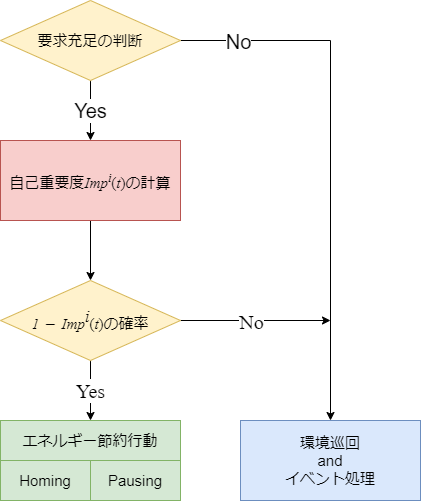
\includegraphics[width=0.6\hsize]{figures/Flowchart.png}
    \caption{エージェントの行動選択}
    \label{fig:flowchart}
  \end{figure}


  \subsection{AMTDS for energy saving and cleanliness (AMTDS/ESC)}
  AMTDSやAMTDS/LD,AMTDS/EDCでは,イベント残存時間をより小さくすることが求められた.
  しかし,エネルギー消費量も同時に小さくすることができればより有用である.
  つまり,イベント残存時間だけではなく,エネルギー消費を節約することが求められることもある.
  したがって,目標決定戦略を選択するQ学習における報酬の計算方法を,式(\ref{eq:reward_AMTDS})から以下の式に変更し,
  報酬を$r_{t_0,t_0+d_{travel}}$とした,AMTDS for energy saving and cleanliness (AMTDS/ESC) \cite{Wu2019}が提案された.
  %
  \begin{equation}
    r_{t_0,t_0+d_{travel}} = \dfrac{\displaystyle\sum_{t_0+1 \leq t \leq t_0+d_{travel}} L_t(v^i_t)}{d_{travel} \times \displaystyle\sum_{t_0+1 \leq t \leq t_0+d_{travel}} E_t(i)}
  \end{equation}
  %
  これにより,エージェントはより少ないエネルギーでより多くのイベントを処理できる目標決定戦略を決定する.
  なお,目標決定戦略$s_{next}$を$\varepsilon$-Greedy法によって決定するのは,\ref{subsec:AMTDS}と同様である. 
  \par

  AMTDS/ESCではさらに,エネルギー節約行動として,HomingとPausingの2つの行動が導入された.
  図\ref{fig:flowchart}はエージェントにおけるエネルギー節約行動にかかわる行動選択のフローチャートである.
  このフローチャートが示すように,2つの条件が満たされた場合,エージェントはエネルギー節約行動を行う.
  その際に,エージェントは2つのエネルギー節約行動のどちらかを行う.
  エージェントは,不要と思われる行動を排除するために,{\em Homing}または{\em Pausing}の2つのエネルギー節約行動をとる.
  以下でそれぞれの詳細を説明する.

  \subsubsection{要求充足の判断}\label{subsec:judge}
  エージェントは,環境の現状を把握し,必要なタスクの品質と比較することで,エネルギー消費を抑える必要がある.
  しかし,どのエージェントも実際の状態を把握することができないため,定期的に推定を行う必要がある.
  そこで,エージェント$i$は,自身が持っている$p^i(v)$を用いて,
  以下の式に従って,時刻$t$における総イベント量$E^i(V_t)$を推定する.
  %
  \begin{equation}\label{eq:fulfill}
    E^i(V_t) = \sum_{v \in V} E^i(L_t(v))
  \end{equation}
  %
  その後,要求条件を満たしているのかを判断するために,以下の式を用いている.
  %
  \begin{equation}\label{eq:requirement}
    E^i(V_t) \leq D_{req}
  \end{equation}
  %
  この式を満たしていれば$i$は自己重要度評価を行い,満たしていなければ,通常の環境巡回とイベント処理を行う.

  \subsubsection{自己重要度評価}
  エージェントは,\ref{subsec:judge}で述べた方法で要求条件を満たしているかを判断し,
  満たしていた場合,自分の貢献度を評価し,自分のエネルギー節約行動が環境の将来に与える影響を予測する.
  そのために,エージェント$i$の時刻$t$における自己重要度$\SelfAss^i(t)$を導入する.
  これは,$i$が協調タスクのために巡回を継続すべきか,エネルギー節約行動をとって巡回を停止すべきかを決定するための,
  $i$の最近の貢献度合いを表している.
  \par

  $SelfAss^i(t)$を計算するために,以下の3つのパラメータを$\forall i\in\AgentSet$に対して定義する.
  %
  \begin{align}\label{eq:param1}
    U^i_s(t_c) &= \frac{\sum_{t_c-T_s < t \leq t_c} L_t(v^i(t))}{T_s}\\
    U^i_l(t_c) &= \frac{\sum_{t_c-T_l < t \leq t_c} L_t(v^i(t))}{T_l}\label{eq:param2}\\
    U^i_f(t_c) &= \frac{\sum_{t_c < t \leq t_c+T_f} E^i(L_t(v^i(t)))}{T_f},\label{eq:param3}
  \end{align}
  %
  ここで,$t_c$は現在の時刻,$T_s$と$T_l~(0 < T_s < T_l)$は過去の短期・長期の評価期間,$T_f$は将来の評価期間,
  $v^i(t)$は$t$において$i$がいた,またはいる予定のノードを表す.
  直感的には,$U^i_s(t_c)$と$U^i_l(t_c)$は過去に$i$が処理したイベント数を表し,
  $U^i_f(t_c)$は将来$t_c+T_f$までに$i$が処理するであろうイベント数の推定値であるといえる.
  つまり,エージェントは以下の2つを考慮して自己重要度を求めている.
  %
  \begin{enumerate}
    \item[(1)] ある期間における過去の貢献度
    \item[(2)] 重要な領域を発見し,その後の行動で多くのイベントを処理できるか
  \end{enumerate}
  %
  なお,式(\ref{eq:param3})でのみ,$L_t(v^i(t))$の代わりに期待値$E^i(L_t(v^i(t)))$が使用されていることに注意されたい.
  \par

  ここで,自己重要度$\SelfAss^i(t)$ ($0 \leq \SelfAss^i(t) \leq 1$)を次の式のように定義する.
  %
  \begin{equation}\label{Imp}
    \SelfAss^i(t) = 
    \begin{cases}
      \; 0                           & (U^i_l = 0\textrm{ のとき} ) \\
      \; \dfrac{U^i_s + U^i_f}{U^i_l} & (U^i_s + U^i_f \leq U^i_l\textrm{ のとき}) \\
      \; 1                           & (\text{その他})
    \end{cases}\\
  \end{equation}
  %
  その後,$i$は以下の式で求められる確率$P^i(t)$でエネルギー節約行動を選択する.
  %
  \begin{equation}\label{pi(t)}
    P^i(t) = 1 - \SelfAss^i(t)
  \end{equation}
  %
  したがって,自己重要度が低いと,エージェントのエネルギー節約行動が促進される.

  \subsubsection{帰還動作 ({\em Homing})}\label{sec:Homing}
  {\em Homing}とは,バッテリ残量にかかわらず,巡回を中止して充電基地に戻ることで,エネルギーを節約する動作のことである.
  エージェント$i$は,充電残量が少なくなり,以下の式を満たしたとき,
  $\HomingCheck$ステップ移動するごとに要求充足度(式(\ref{eq:fulfill}))をチェックする.
  %
  \begin{equation}
    \BatteryLevel^i(t) < \HomingBattery\cdot\BatteryMax
  \end{equation}
  %
  ここで,正の整数$HomingCheck$は{\em Homing}による頻繁な充電基地への帰還を避けるためのパラメータ,
  $\HomingBattery$ ($0 < \HomingBattery < 1$)はバッテリ残量低下を判断するためのパラメータである.
  式(\ref{eq:fulfill})を満たさない場合,$i$は巡回を継続し,
  満たす場合は,確率$P_i(t)$で$i$が現在の$v^i_{tar}$を$v_{charge}$に変更する{\em Homing}を行い,
  充電基地についたら充電を行う.
  また,{\em Homing}中はイベント処理は行うが,要求充足の判定や自己重要度の計算は行わない.
  なお,充電基地から遠い地点を巡回しているエージェントがこのチェックをする前に充電基地に帰還することもありうる.

  \subsubsection{待機動作 ({\em Pausing})}\label{sec:Pausing}
  {\em Pausing}とは,充電完了後,エージェントはすぐに巡回を再開せずに,待機する動作のことである.
  エージェント$i$が時刻$t$に充電が完了したとき,要求充足度(式(\ref{eq:fulfill}))をチェックし,
  満たす場合は一定の休止時間$\PausingInt$ステップ充電基地で待機する.
  満たさない場合は,巡回を再開する.
  

  \section{提案手法}
  AMTDS/ESCでは,要求値$\Dreq$とエネルギー節約行動の導入によって,
  品質要求を満たしつつ,エネルギー消費量を削減することができた.
  しかし,{\em Homing}と{\em Pausing}の2つのエネルギー節約行動のうち,どちらか片方しか行うことができなかった.
  また,全てのエージェントが同一の視点で要求充足の判断を行っていたため,
  環境の状態の推定が不十分であり,要求条件を満たす上で不必要な巡回を行っているため,
  エネルギーを余分に消費してしまっている.
  これらの問題を解消するため,本研究では,
  AMTDS for energy saving under the requirement (AMTDS/ER)と,
  AMTDS/EDCに加えたAMTDS for energy saving under the requirement with communications (AMTDS/ERC)
  を提案する.
  以下では,ベースとしている手法との違いに絞って説明する.
  
  \subsection{AMTDS for energy saving under the requirement (AMTDS/ER)}
  この節では,AMTDS/ESCをベースに,エージェントがそれぞれの視点で将来の環境状態を予測する方法を学習し,
  充電基地についた際に,未来の環境状態を予測し,待機時間を動的に決定する手法である,AMTDS/ERについて説明する.
  また,品質要求を満たした上で,不要なエージェントを停止する2通りの手法についても説明する.  

  \subsubsection{未来のイベント量の予測}\label{sec:predict}
  AMTDS/ERでは,\ref{sec:changeEnergySaving}項で詳しく説明するが,
  {\em Pausing}による待機時間を可変に変更する.
  その際に,未来のイベント量の予測をする必要があるため,その方法について説明する.
  \par

  エージェント$i$は,将来の時刻$t_c+T$における$\forall v\in V$の期待値$E^i(L_{t_c+T}(v))$を,
  以下の式に従って求める.
  %
  \begin{equation}\label{eq:estimation}
    E^i(L_{t_c+T}(v)) = p(v) \times \{(t_c+T)-t^v_{vis}\}
  \end{equation}
  %
  ここで,$T>0$は$i$がどの程度先の未来を推定するかを指定するパラメータである.
  
  \subsubsection{予測の自律的補正学習}
  \ref{sec:predict}項で説明した未来のイベント量の予測を行った後,
  エージェント$i$は式(\ref{eq:fulfill})を確認する.
  しかし,この式(\ref{eq:fulfill})は$T$に対して単調増加であるため,
  この推定は,均一な作業量に基づく理想的な場合であり,
  他エージェントによる努力(巡回)は無視されている.
  特に,$i$がエネルギー節約や充電のために巡回を停止していても,
  他エージェントは要求値$\Dreq$を維持しようとする.
  さらに,各エージェントは異なる特徴を持つ場所を訪問するため,
  他エージェントによる努力は,個々の視点によって明らかに異なる.
  したがって,エージェントは,エネルギー節約行動中における他エージェントの
  努力の可能性を学習する必要がある.
  \par

  これを調整するために,学習パラメータ$K^i$を$\forall i\in \AgentSet$に導入する.
  そして,エージェント$i$は,式(\ref{eq:fulfill})の代わりに,
  以下の式を用いて要求条件を満たしているかを判断する.
  % 
  \begin{equation}\label{eq:revised}
    \sum_{v \in V} E^i(L_{t_c+T}(v)) \div K^i \leq \Dreq
  \end{equation} 
  %
  さらに,$K^i$は個々に次の式に従って更新される.
  %
  \begin{equation}\label{eq:ParameterK}
    \begin{cases}
      K^i \gets (1 - \alpha_k) \times K^i + \alpha_k \times \dfrac{\Dreq}{E^i(D_t)}
      K^i & (E^i(D_t) \leq \Dreq \textrm{ のとき})\\
      K^i \gets K^i - \left( \dfrac{E^i(D_t)}{\Dreq} - 1 \right) 
      & (E^i(D_t) > \Dreq \textrm{ のとき})
    \end{cases}
  \end{equation}
  %
  ここで,$t$におけるイベント量の推定値は$E^i(D_t)=\sum_{v\in V} E^i(L_t(v))$で定義され,
  $\alpha_k>0$は学習率である.
  $K^i$がいつ更新されるかは,\ref{sec:changeEnergySaving}項で説明する.


  \begin{algorithm}
    \caption{{\sf PLength}: To decide pausing time-length.}\label{alg:PausingTime}
    \begin{algorithmic}[1]
      \REQUIRE $\PausingInt > 0$, $\PauseTimeFactor=0$, $T_\PauseTimeFactor > 0$
      \WHILE {$\PauseTimeFactor \leq T_\PauseTimeFactor$} 
      \STATE $T\leftarrow (\PauseTimeFactor+1)\cdot\PausingInt$ // $T$ is
      used in Formula~(\ref{eq:revised})
      \IF {Formula~(\ref{eq:revised}) holds}
      \STATE $\PauseTimeFactor \leftarrow \PauseTimeFactor+1$
      \ELSE
      \STATE break
      \ENDIF
      \ENDWHILE
      \STATE // エージェントは待機時間$\PauseTimeFactor\cdot\PausingInt$の{\em Pausing}を行う
      \STATE // もし$\PauseTimeFactor=0$の場合, エージェントは即座に充電基地を出発し,巡回を再開する
      \STATE return $\PauseTimeFactor\cdot\PausingInt$.
    \end{algorithmic}
  \end{algorithm}


  \subsubsection{エネルギー節約行動の修正}\label{sec:changeEnergySaving}
  ここでは,より多くのエネルギーを削減するための,
  \ref{sec:Homing}項と\ref{sec:Pausing}項で説明したエネルギー節約行動の修正点について説明する.
  AMTDS/ESCでは,時刻$t$に充電が完了すると,エージェント$i$が要求条件(式(\ref{eq:fulfill}))を満たす場合,
  $i$は固定の待機時間$PausingInt$ステップ{\em Pausing}を行っていた.
  \par

  しかし,提案手法では,エージェントは推定状態の条件に応じて可変の待機時間をとる.
  $i$は以下で説明する可変長の{\em Pausing}を確率$P_i(t)$で行い,$t$で充電を完了する.
  ただし,例外として,$i$は{\em Homing}によって充電基地$v_{base}$に戻ったときのみ,
  $P_i(t)$を計算せずに,常に可変長の{\em Pausing}を行う.
  これは,{\em Homing}のみでは,エージェントによる,「イベント処理$\rightarrow$充電$\rightarrow$イベント処理$\rightarrow\cdots$」
  のサイクルが短縮しただけで,エネルギー消費量にはあまり影響しない.
  既に環境が要求条件を満たしていて,自分は余力があっても充電基地に戻るべきと判断し{\em Homing}を行っているため,
  {\em Pausing}を行うことは自然であり,エネルギー消費量の減少が見込める.
  \par

  可変長の{\em Pausing}について説明する.
  まず,$i$は待機時間を以下のように決定する(Algorithm~\ref{alg:PausingTime}の\textsf{PLength}参照).
  初期状態では,エージェント$i$は$\PauseTimeFactor=0$,$T=\PausingInt$と設定する.
  時刻$t$にバッテリが満充電になると,$i$は要求充足度をチェックし(式(\ref{eq:revised})),
  満たしていない場合は,$i$は直ちに充電基地から出発し,巡回を再開する.
  つまり,待機時間は0となる.
  満たしている場合は,$\PauseTimeFactor$を1だけインクリメントし,
  $T \leftarrow (\PauseTimeFactor+1)\cdot \PausingInt$とセットする.
  次に,$i$は再び要求度をチェックし,待機時間を決定するか,
  $\PauseTimeFactor=T_\PauseTimeFactor$となるまでこの操作を繰り返す.
  ただし,$T_\PauseTimeFactor$はこの反復の最大値である.
  その後,$i$は$\PauseTimeFactor\cdot\PausingInt$ステップだけ{\em Pausing}を行う.
  エージェントはこの可変長の{\em Pausing}の後は,必ず充電基地を出発する.
  \par

  前述したように,エージェント$i$が{\em Homing}で充電基地に戻る場合,AMTDS/ESCとは異なり,
  充電完了後に必ず可変長の{\em Pausing}を行う.
  この際に,上記のアルゴリズムによって待機時間が0になる可能性もなる.
  以下では,可変長の{\em Pausing}を単に{\em Pausing}と呼ぶ.

  \subsection{不要なエージェントの停止}\label{sec:deactivation}
  エネルギー消費抑制の観点からは,要求条件を満たした上で,環境巡回に必要なエージェント数が十分であれば,
  たとえ必要最小数までではなくとも,エージェントを一時的に休止するだけでなく,
  一部のエージェントの巡回を停止することが有効である.
  さらに,これらの停止したエージェントは,他の場所で使えたり,エージェントが故障した場合のバックアップとして使用することができる.
  しかし,複雑でイベント発生確率の分布が一様でない環境では,どのエージェントを停止すれば要求条件を満たしたままでいられるかや,
  どれだけのエージェントが必要かを事前に把握することは困難である.
  \par

  \ref{sec:expAnalsis}項で詳細に説明するように,$K^i$はエージェントによって大きなばらつきがあり,
  大きく分けて2つのグループに分かれていることが分かった.
  特に,$K^i$が比較的大きいグループに属するエージェントは,エネルギー消費を抑えるために比較的長い時間{\em Pausing}を行っていたため,
  このような$K^i$が最も大きいエージェント$i_{de}\in\AgentSet$を停止させる手法を提案する.
  %
  \begin{equation}
    i_{de} = \argmax_{i\in\AgentSet} K^i
  \end{equation}
  %
  その後,いくつかのエージェントの$K^i$がまだ大きい場合,
  品質要求が満たされているのならば,
  全てのエージェントの$K^i$が相対的に小さくなるまで同様の停止処理を繰り返す.
  ここで,\ref{ex:ER4}項で詳細に説明するように,$K^i$の降順にエージェントを停止することによって,
  停止による$D(s)$の一時的な悪化を防いでいる.
  \par

  本実験では,不要なエージェントの停止手法として,
  関数\textsf{PLength}が呼び出された回数を比較して停止する手法(Deactivation on Count)と,
  エージェントの待機時間を比較して停止する手法(Deactivation on Time)の2つの手法を提案する.
  \\ \red{英語名については要検討}\\

  \subsubsection{Deactivation on Count}\label{sec:CountStop}
  システムは$\DeactCheckInterval>0$ステップごとに,関数\textsf{PLength}が全てのエージェントによって
  呼び出された回数である$\PauseCount$をカウントし,$\PauseCount$と$K^{i_{de}}$が大きい場合,
  すなわち,以下の式を満たすかを確認する.
  %
  \begin{equation}
    \PauseCount \geq \DeactCount \textrm{ and } \max_{i\in\AgentSet}
    K^i \geq \DeactThreshold,
  \end{equation}
  %
  この式を満たす場合,$i_{de}$は停止する.
  ここで,$\DeactThreshold > 0$は停止の閾値を示し,
  $\DeactCount$はシステムから見て,最近の$\DeactCheckInterval$の間に
  複数の{\em Pausing}が試みられたかどうかを判断する閾値を示す.
  ここで,関数\textsf{PLeangth}によって$\PauseTimeFactor=0$の場合でもカウントすることに注意されたい.
  これは,$\PauseCount$と$\DeactCount$の式は,要求品質をみたす際に現在どの程度余裕があるのかを確認している.
  図\ref{fig:flowchart}より,{\em Homing}や{\em Pausing}を行うということは,
  現在は品質要求を満たしているとエージェントが判断しているため,このようなカウント方法にしている.
  

  \begin{figure}
    \centering
    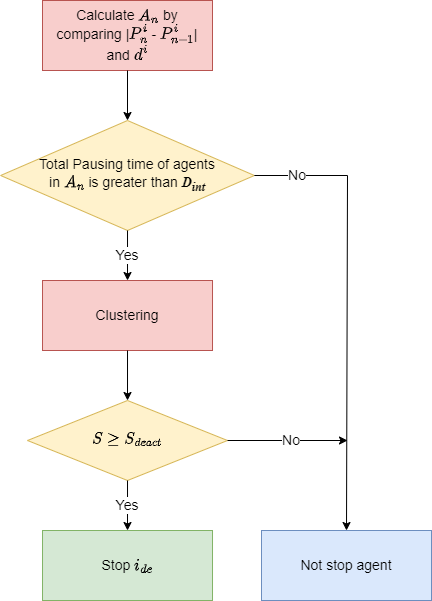
\includegraphics[width=0.6\hsize]{figures/Flowchart_stop_E.png}
    \caption{エージェントの停止選択}
    \label{fig:flowchart_stop}
  \end{figure}


  \subsubsection{Deactivation on Time}\label{sec:TimeStop}
  \ref{sec:expAnalsis}項で詳細に説明するように,AMTDS/ERでは,イベント処理中心のグループと,
  エネルギー節約中心のグループの2グループに分かれる.
  Deactivation on Timeは,その性質とエージェントの待機時間を用いて停止するか否かを判断する手法である.
  \par
  
  まず,エージェント$i$の待機時間の通常変化量$d^i$を導入する.
  エージェントごとに待機時間の変化量は異なり,これを学習することにより,
  $i$が品質要求を考慮して待機時間を変化させている途中なのか,
  均衡状態なのかを判断できるようになる.
  これを式(\ref{eq:learnInterval})のように$\DeactCheckInterval$に対して$\beta_s(\beta_s > 1)$で割ったステップ数である,
  $\DeactLearnInterval$ステップごとに式(\ref{eq:ParameterD})に従って更新する.
  %
  \begin{equation}\label{eq:learnInterval}
    \DeactLearnInterval = \dfrac{\DeactCheckInterval}{\beta_s}
  \end{equation}
  %
  %
  \begin{equation}\label{eq:ParameterD}
    d^i \gets \alpha_d \times |T^i_n - T^i_{n-1}| + (1-\alpha_d) \times d^i
  \end{equation}
  %
  ここで,$T^i_n$は全ての正整数$n$について,
  $(n-1) \times \DeactLearnInterval \sim n \times \DeactLearnInterval$ステップでの$i$の総待機時間である.
  つまり,$|T^i_n - T^i_{n-1}|$とは,$\DeactLearnInterval$ステップごとの総待機時間の変化量を表す.
  さらに,$\alpha_l$は学習率であるが,これは以下の式に従って,2通りの値をとる($\alpha_1 > \alpha_2$).
  %
    \begin{equation}
      \alpha_d = 
      \begin{cases}
        \alpha_1 & (|T^i_n - T^i_{n-1}| \leq d^i \textrm{のとき}) \\
        \alpha_2 & (|T^i_n - T^i_{n-1}| > d^i \textrm{のとき})
      \end{cases}
    \end{equation}
  %  
  \par

  図\ref{fig:flowchart_stop}は,Deactivation on Timeでの停止をするかどうかの判断のフローチャートである.
  $(n-1) \times \DeactCheckInterval \sim n \times \DeactCheckInterval$ステップでの$i$の総待機時間である
  $P^i_n$を用いて,$\DeactCheckInterval$ステップごとに$|P^i_n - P^i_{n-1}|$と$\beta_s \times d^i$を比較する.
  $|P^i_n - P^i_{n-1}| \leq d^i$のエージェントの集合を$A_n$として,以下の式を満たすか確認する.
  %
  \begin{equation}\label{eq:checkD}
    \sum_{i \in A_n} P^i_n \geq \DeactCheckInterval
  \end{equation}
  %
  この式を満たせば,$i_{de}$を停止後も残りのエージェント達は,
  少なくとも$(\DeactLearnInterval-P^{i_{de}}_n)$ステップ待機しているため,
  この待機時間を減らすことで$i_{de}$の分のイベント処理をカバーできる.
  また,式(\ref{eq:ParameterD})で$\alpha_d$が2通りの値をとる理由は,
  $\alpha_d$が固定の場合,$\DeactCheckInterval > \DeactLearnInterval$より,
  $i$が待機時間を変化中の時でも直前の数回の更新で$d^i$に影響を与え,大きな値となってしまう.
  これにより,本当は待機時間を変更させているのに式(\ref{eq:checkD})を満たしてしまう恐れがある.
  これを防ぐために,$\alpha_d$は2通りの値をとり,$\alpha_1 > \alpha_2$としている.
  さらに,エージェントを停止していき,エージェント数が少なくなっていくと,
  品質要求を満たすために,待機時間が大きかったエージェントも,
  イベント処理を多く行うために待機時間を小さくしていかなければならない.
  最終的に,このエージェントの待機時間が0になり,
  品質要求を満たす上でこれ以上エージェントを停止できなかったはずなのに停止してしまい,
  残りのエージェント数では,全力でイベント処理を行っても品質要求を満たせないということは避けなければならない.
  そのため式(\ref{eq:checkD})では,$\AgentSet$の総待機時間ではなく,
  待機時間が均衡状態であるエージェントの集合である$A_n$の総待機時間を用いている.
  \par

  さらに,全ての巡回エージェントの$K^i$と$P^i_n$をそれぞれ平均0,標準偏差1に標準化し,
  k-means法により2つのクラスターにクラスタリングする.
  その後,以下の方法で$i$のシルエット係数$s^i$を計算し,それの平均シルエット係数$S$を求める.
  %
  \begin{enumerate}
    \item[(1)] クラスタ内の凝集度として,$i$が属するクラスタ$C_{in}$の他の点までの平均距離$c^i_{in}$を計算
    \item[(2)] 別クラスタからの乖離度として,$i$が属しないクラスタ$C_{out}$に属する点までの平均距離$c^i_{out}$を計算
    \item[(3)] 以下の式に従って,$i$のシルエット係数$s^i$を計算
              %
                \begin{equation}
                  s^i = \dfrac{c^i_{out} - c^i_{in}}{(\max(c^i_{in}, c^i_{out}))}
                \end{equation}
              %
  \end{enumerate}
  %
  なお,$C_{in}$に属するエージェントが$i$しかいない場合,$c^i_{in} = 0$とする.
  このようにして求めた$S$を用いて,以下の式を満たすか確認する.
  %
    \begin{equation}\label{eq:sillet}
      S \geq S_{deact}
    \end{equation}
  %
  ここで,$S_{deact}$平均シルエット係数の閾値である.
  一般に,シルエット係数は,複数のクラスターに対して計算し,
  最適なクラスター数を決めるために用いられる.
  しかし,\ref{sec:expAnalsis}項で詳細に説明するように,
  提案手法のAMTDS/ERは,エージェントを2つのグループに分けることができる.
  この2つのグループに分かれる前,つまりエージェントの役割分担がしっかり行われる前に
  停止を行わないようにするため,本来の使用用途とは異なるが式(\ref{eq:sillet})のように
  シルエット係数を用いている.
 
  \subsection{AMTDS for energy saving under the requirement with communications (AMTDS/ERC)}
  \red{subsectionなどの構成も含めて再考}\\
  この節では,従来手法のAMTDS/EDCと,AMTDS/ERを組み合わせた手法である.
  しかし,AMTDS/EDCにエネルギー節約行動や学習パラメータ$K^i$を導入しただけではうまくいかない.
  それの一番大きな理由は,AMTDS/ERでは既知であったイベント発生確率を学習し,
  さらにそれを\ref{sec:AMTDS/EDC}で述べたように,
  交渉を行うため,その値はエージェントによって異なる.
  そのため,AMTDS/ERのように,式(\ref{eq:estimation})では実際の総イベント量との差が大きい.
  つまり,現在の環境全体のイベント量を予測することが困難になった.
  これを解決するため,以下で説明する変更・工夫を行った.
  なお,$p^i(v)$の学習のため,エネルギー節約行動は$T_{hp}$ステップから開始する.
  
  \subsubsection{学習パラメータ$C^i_{rate}$の導入}
  まず,エージェント$i$のイベント発生確率の学習がどの程度ずれているのかを示す学習パラメータ$C^i_{rate}$を導入する.
  $i$は充電基地を出発時に,イベントの期待値の総和$S^i_{est}$と実測値の総和$S^i_{real}$を0にリセットする.
  時刻$t$にノード$v \in V^i_R$を訪問した際に,
  期待値$E^i(L_t(v))$の計算とイベント処理による実測値$L_t(v)$の取得を行い,
  それぞれを$S^i_{est}$と$S^i_{real}$に加算する.
  その後,充電基地に戻った際に,以下の式に従って$C^i_{rate}$を更新する.
  %
    \begin{equation}
      C^i_{rate} \gets \alpha_{rate} \times \dfrac{S^i_{real}}{S^i_{est}} + (1-\alpha_{rate}) \times C^i_{rate}
    \end{equation}
  %
  
  \subsubsection{$K^i$の更新方法の変更}
  $C^i_{rate}$の導入に伴い,$K^i$の更新方法も式(\ref{eq:ParameterK})から変更する.
  まず,以下の式から
  %
  \begin{equation}\label{eq:ParameterK/ERC}
    K^i \gets (1 - \alpha_k) \times K^i + \alpha_k \times \dfrac{\Dreq}{E^i(D_t(V^i_R)) \times C^i_{rate}}
  \end{equation}
  %
  ここで,$i$の$t$における総イベント量の推定値$E^i(D_t(V^i_R))$は,
  $V$から壁などの障害物を表すノードを除いたノード集合$V_{access}$と$V^i_R$を用いて,以下の式に従って求められる.
  %
    \begin{equation}
      E^i(D_t(V^i_R))=\sum_{v\in V^i_R} E^i(L_t(v)) \times \dfrac{|V_{access}|}{|V^i_R|}   
    \end{equation}
  %

  \subsubsection{未来のイベント量の予測の変更}
  AMTDS/ERでは,式(\ref{eq:estimation})を用いて$T$ステップ後のイベント量を予測していたが,
  AMTDS/ERCではイベント発生確率が実際とは異なるため,
  このままでは品質要求を満たせなくなってしまう可能性がある.
  そのため,未来のイベント量の予測を$C^i_{rate}$を用いて以下の式に変更した.
  %
  \begin{equation}
    E^i(L_{t_c+T}(v)) = p(v) \times \{(t_c+T)-t^v_{vis}\} \times \dfrac{|V_{access}|}{|V^i_R|} \times C^i_{rate}
  \end{equation}
  %
  

  \begin{table}
    \begin{minipage}[t]{.55\textwidth}
      \centering
      \caption{エージェントに関するパラメータ}
      \begin{tabular}{lcr} \\ \hline
        種類 & パラメーター & 値 \\ \hline
        エージェント数 &  $\vert A \vert$ & 20 \\ \hline
        バッテリ & $B^i_{max}$ & 900 \\
                   & $B^i_{drain}$ & 1 \\
                   & $k^i_{charge}$ & 3 \\ \hline
        経路生成戦略 & $d_{myopia}$ & 10 \\
                     & $k_{att}$ & 1.0 \\
                     & $k_{rover}$ & 1.2 \\ \hline
      \end{tabular}
      \label{tb:1}
    \end{minipage}
    %
    \hfill
    %
    \begin{minipage}[t]{.55\textwidth}
      \centering
      \caption{目標決定戦略のパラメータ}
      \begin{tabular}{lcrr} \\ \hline
        目標決定戦略 & パラメーター & 値 \\ \hline
        PGS & $N_g$ & 5 \\ \hline
        PI & $N_i$ & 5 \\ \hline
        BNPS & $\alpha$ & 0.1 \\
             & $d_{rad}$ & 15 \\ \hline
        AMTDS & $\alpha$ & 0.1 \\
              & $\varepsilon$ & 0.05 \\ \hline
        AMTDS/LD & $\beta$ & 0.1 \\ \hline 
        AMTDS/EDC & $N_{gmax}$ & 100 \\
                  & $N_{cmax}$ & 10 \\
                  & $T_c$ & 0.05 \\
                  & $\gamma$ & 10 \\
                  & $\delta$ & 0.5 \\ \hline
      \end{tabular}
      \label{tb:2}
    \end{minipage}
    %
    \vskip\baselineskip
    %
    \begin{minipage}[t]{.55\textwidth}
      \centering
      \caption{エネルギー節約行動に関するパラメータ}
      \begin{tabular}{lcrr} \\ \hline
        種類 & パラメーター & 値 \\ \hline
        自己重要度評価 & $T_s$ & 20 \\
                      & $T_l$ & 50 \\
                      & $T_f$ & 10 \\ \hline
        {\em Homing} & $\HomingCheck$ & 100 \\
               & $k_{homing}$ & $1/3$ \\ \hline
        {\em Pausing} & $\PausingInt$ & 100 \\
                & $T_\PauseTimeFactor$ & 1,000 \\ \hline  
        AMTDS/ER & $\alpha_k$ & 0.1 \\ \hline
        AMTDS/ERC & $T_{hp}$ & 1,000,000 \\
                  & $\alpha_{rate}$ & 0.1 \\ \hline       
      \end{tabular}
      \label{tb:3}
    \end{minipage}
    %
    \hfill
    %
    \begin{minipage}[t]{.55\textwidth}
      \centering
      \caption{エージェントの停止に関するパラメータ}
      \begin{tabular}{lcrr} \\ \hline
        種類 & パラメーター & 値 \\ \hline
        Deactivation on Count & $\DeactCheckInterval$ & 250,000 \\
                                & $\DeactCount$ & 100 \\
                                & $\DeactThreshold$ & 1.0 \\ \hline
        Deactivation on Time & $\DeactCheckInterval$ & 250,000 \\
                              & $\beta_s$ & 10 \\
                              & $\alpha_1$ & 0.1 \\
                              & $\alpha_2$ & 0.05 \\
                              & $S_{deact}$ & 0.7 \\ \hline
        \end{tabular}
      \label{tb:4}
    \end{minipage}
  \end{table}

  
  \section{評価実験}
  この章では,提案手法である,AMTDS/ERやAMTDS/ERCと,
  エージェントがエネルギー節約行動をとらない手法であるAMTDS\cite{Yoneda2013}とAMTDS/EDC\cite{Sugiyama2019}や,
  エージェントがエネルギー節約行動を調整するパラメータを学習しない手法であるAMTDS/ESC\cite{Wu2019}を比較する実験を行い,
  提案手法の有効性を検証する.
  評価指標$D(s)$と$C(s)$を調査することにより,提案手法が他の手法と比べて,
  エージェントが品質要求を満たしつつ,エネルギー消費を削減できることを実証する.
  また,$\forall i\in\AgentSet$の$K^i$の分布を分析し,その値に応じてエージェントを2つのグループに分けた.
  さらに,要求値$\Dreq$を変化させたときのエージェントの対応を検証も行う.
  加えて,エージェントの停止を行う際に,停止方法による要求充足度の違いを検証し,
  それを基に,品質要求を満たしながら巡回エージェントの数を減らすことができることを実証する.
  実験に用いたパラメータ値を表\ref{tb:1}$\sim$\ref{tb:3}に示す.


  \begin{figure}
    \begin{minipage}{0.45\hsize}
      \centering
      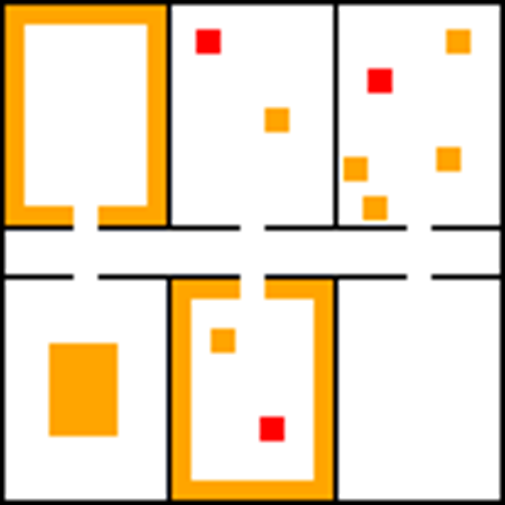
\includegraphics[width=1.0\hsize]{figures/Graph_Office.png}
      \subcaption{環境1}
      \label{subfig:env1}
    \end{minipage}
    \hfill
    \begin{minipage}{0.52\hsize}
      \centering
      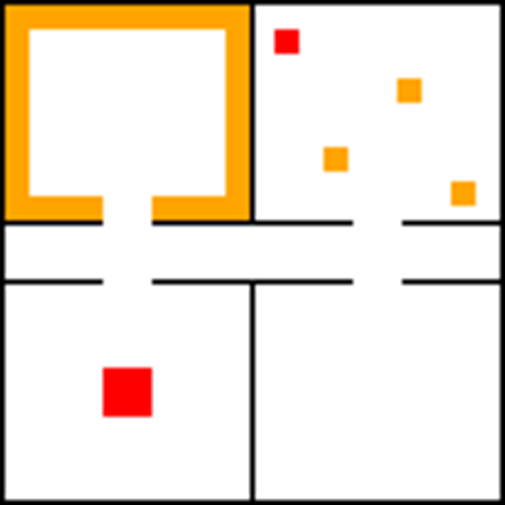
\includegraphics[width=0.865\hsize]{figures/Graph_Complex.png}
      \subcaption{環境2}
      \label{subfig:env2}
    \end{minipage}
    \caption{実験環境}\label{fig:env}
  \end{figure}


  \subsection{実験環境}
  本研究では,図\ref{fig:env}に示すように,
  大きさが$101 \times 101$の2次元グリッド環境を2つ用意した.
  図\ref{subfig:env1}の環境$G_1=(V_1, E_1)$は,比較のため\cite{Wu2019}の実験で用いられていた環境と同じである.
  この環境は,6つの独立した部屋と,それらをつなぐ廊下が中央にある.
  黒線は壁(エージェントが通過できない障害物)を表す.
  各ノード$v \in V_1$は$(x_v, y_v)$の整数座標で表され,$-50 \leq x_v,y_v \leq 50$である.
  図\ref{fig:env}の色に従って,ノード$\forall v\in V_1$のイベント発生確率$p(v)$を次のように設定した.
  %
  \begin{equation}
    p(v) = 
    \begin{cases}
      10^{-3}\ & \textrm{($v$が赤色の領域内の場合)}\\
      10^{-4}\ & \textrm{($v$がオレンジ色の領域内の場合)}\\
      10^{-6}\ & \textrm{($v$が白色の領域内の場合)}\\
    \end{cases}
    \label{eq:prob}
  \end{equation}
  %
  したがって,色が濃いほどイベント発生確率は高くなる.
  \par

  図\ref{subfig:env2}の環境$G_2=(V_2, E_2)$は4つの部屋があるが,各部屋の大きさは少し広くなっている.
  イベント発生確率も図\ref{subfig:env1}と同様に,色を使って式(\ref{eq:prob})で指定する.
  この環境は図\ref{subfig:env1}と比べると,イベント発生確率の総和は少ないが,
  その分エージェントがエネルギー節約行動を行う必要がある.
  \par
  
  エージェント数$\vert \AgentSet \vert$は20であり,全てのエージェントの充電基地は中心$(0, 0)$に配置する.
  エージェントはバッテリを満タンにしてから充電基地を出発し,周囲を巡回して,
  バッテリ残量が0になる前に充電基地に戻るというサイクルを繰り返す.
  また,バッテリの性能を$(B^i_{max}, B^i_{drain}, k^i_{charge}) = (900, 1, 3)$とする.
  したがって,0から充電が完了するまでの時間は2700ステップとなり,最大活動時間は3,600ステップとなる.
  これにより,$D(s)$と$C(s)$のデータ収集間隔$t_e - t_s$を3,600とした.
  さらに,品質要求値を$\Dreq=600$とし,学習パラメータ $K^i$の初期値を1.0とした.
  \par

  本実験では,1回の試行ステップ数は評価実験によって異なるが,全ての評価実験の$D(s)$と$C(s)$の値は,
  独立した50回の試行による平均値である.

  \subsection{AMTDS/ERについての実験結果・考察}\label{result_ER}
  提案手法であるAMTDS/ERについての評価実験を,エネルギー節約行動を行わないAMTDSや,
  エネルギー節約行動を調整するパラメータを学習しないAMTDS/ESCと比較しながら行った.
  この節では,複数の条件下での実験結果を,評価指標である$D(s)$や$C(s)$,さらには,必要に応じて他の指標とも比較していく.

  
  \begin{figure}
    \centering
    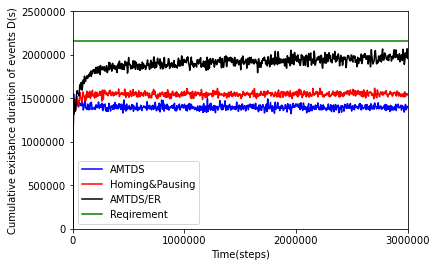
\includegraphics[width=0.9\hsize]{figures/ds_graph_3600_ave_ER_Office_600.png}
    \caption{$D(s)$の時間推移(実験1)}
    \label{fig:ds_ER_Office}
    \vspace{12pt}
    \centering
    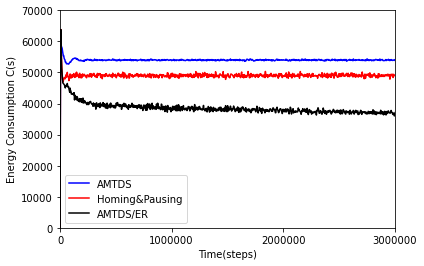
\includegraphics[width=0.9\hsize]{figures/cs_graph_3600_ave_ER_Office_600.png}
    \caption{$C(s)$の時間推移(実験1)}
    \label{fig:cs_ER_Office}
  \end{figure}
  

  \subsubsection{実験1: 性能評価}\label{ex:ER1}
  図\ref{fig:ds_ER_Office},\ref{fig:cs_ER_Office}は,環境1で実験を行い,
  それぞれ3,600ステップごとのイベント残存時間の総和$D(s)$と,エージェントの総エネルギー消費量$C(s)$の時間推移を示したものである.
  なお,図\ref{fig:ds_ER_Office}では,$\Dreq=600$なので,エージェントは$D(s)\leq 2,160,000$ ($=3,600\Dreq$)を保つことが
  要求条件であることに注意されたい.
  図\ref{fig:ds_ER_Office}に示すように,全ての手法が品質要求を満たしていることがわかる.
  特に,従来手法であるAMTDSとAMTDS/ESCは,$D(s)$が要求値よりもかなり小さい値を維持している.
  \par

  しかし,これは要求値以上の巡回による過剰なエネルギー消費を示唆しており,
  これを図\ref{fig:cs_ER_Office}で確認することができる.
  この図から,提案手法AMTDS/ERは,AMTDSに比べて$D(s)$は約$40.3\%$増加しているが,
  $C(s)$を約$30.9\%$削減することができた.
  なお,このデータは2,000,000ステップから3,000,000ステップの平均値である.
  AMTDS/ESCもエネルギー消費量を削減することはできたが,その削減効果は限られており,
  AMTDS/ERはAMTDS/ESCよりも,$D(s)$を約$26.2\%$増加させ,$C(s)$を約$24.0\%$削減することができた.
  これは,学習パラメータ$K^i$の導入により,各エージェントがエネルギー節約行動中の他のエージェントの巡回による効果を,
  ある程度予測できるようになったためであると考えられる.


  \begin{figure}
    \centering
    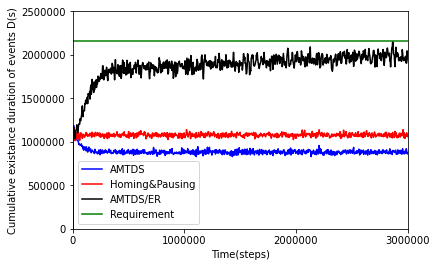
\includegraphics[width=0.9\hsize]{figures/ds_graph_3600_ave_ER_Complex_600.png}
    \caption{$D(s)$の時間推移(実験2)}
    \label{fig:ds_ER_Complex}
    \vspace{12pt}
    \centering
    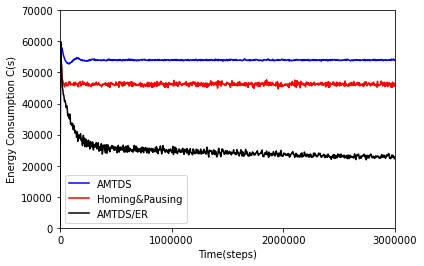
\includegraphics[width=0.9\hsize]{figures/cs_graph_3600_ave_ER_Complex_600.png}
    \caption{$C(s)$の時間推移(実験2)}
    \label{fig:cs_ER_Complex}
  \end{figure}
  

  \subsubsection{実験2: 異なる環境による性能評価}\label{ex:ER2}
  図\ref{fig:ds_ER_Office},\ref{fig:cs_ER_Office}は,環境2で実験を行い,
  それぞれ3,600ステップごとの$D(s)$と$C(s)$の時間推移を示したものである.
  実験2でも,実験1と同様な結果がみられる.
  前述のように,環境2では,イベント発生確率の総和は環境1よりはるかに小さく,
  エージェントは実験1よりも多くのエネルギーを削減するために,
  より多くのエネルギー節約行動を行うことができるかを確認する.
  図\ref{fig:ds_ER_Complex}と図\ref{fig:cs_ER_Complex}より,エージェントは,
  要求条件を満たしながらエネルギー節約行動を徐々に増加させ,エネルギー消費を削減したことが分かり,
  期待通りの行動をとることができた.
  これにより,AMTDS/ERはAMTDS/ESCよりも,エネルギーを約半分しか消費していないことが分かる.


  \begin{figure}
    \begin{minipage}{1.0\columnwidth}
      \centering
      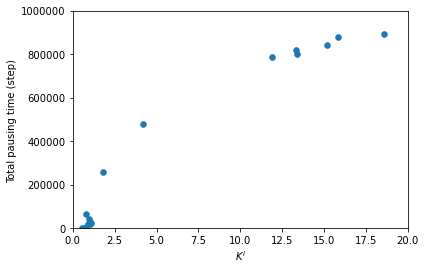
\includegraphics[width=0.8\hsize]{figures/CorrectionScatter_Office_ER.png}
      \caption{エージェントごとの$K^i$と待機時間の関係(実験1)}
      \label{fig:cscatter_ER_Office}
    \end{minipage}
    \\[40pt]
    \begin{minipage}{1.0\columnwidth}
      \centering
      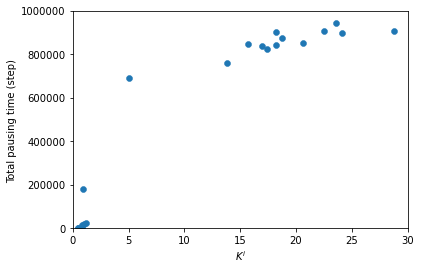
\includegraphics[width=0.8\hsize]{figures/CorrectionScatter_Complex_ER.png}
      \caption{エージェントごとの$K^i$と待機時間の関係(実験2)}
      \label{fig:cscatter_ER_Complex}
    \end{minipage}
  \end{figure}

  \begin{figure}
    \begin{minipage}[t]{0.48\columnwidth}
      \centering
      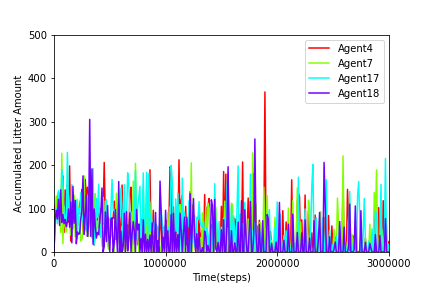
\includegraphics[keepaspectratio, width=\linewidth]{figures/al_graph_ER_Office_top.png}\\
      \subcaption{$K^i$の上位4体}
      \label{fig:al_ER_Office_top}
    \end{minipage}
    \hfill
    \begin{minipage}[t]{0.48\columnwidth}
      \centering
      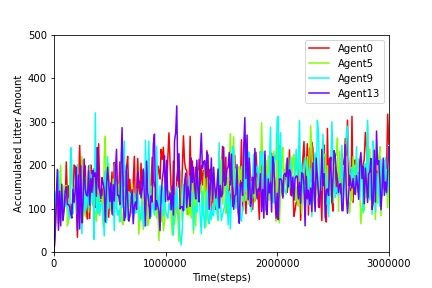
\includegraphics[keepaspectratio, width=\linewidth]{figures/al_graph_ER_Office_worst.png}\\
      \subcaption{$K^i$下位4体}
      \label{fig:al_ER_Office_least}
    \end{minipage}
    \caption{エージェントごとのイベント処理量の時間推移(実験1)}
    \label{fig:al_ER_Office}
  \end{figure}~\begin{figure}[t]
      \begin{minipage}[t]{0.48\columnwidth}
        \centering
        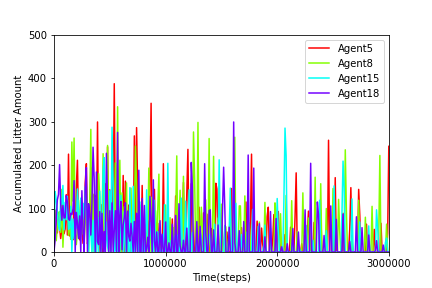
\includegraphics[keepaspectratio, width=\linewidth]{figures/al_graph_ER_Complex_top.png}\\
        \subcaption{$K^i$上位4体}
        \label{fig:al_ER_Complex_top}
      \end{minipage}
    \hfill
      \begin{minipage}[t]{0.48\columnwidth}
        \centering
        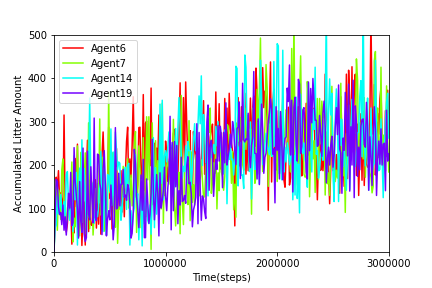
\includegraphics[keepaspectratio, width=\linewidth]{figures/al_graph_ER_Complex_worst.png}\\
        \subcaption{$K^i$下位4体}
        \label{fig:al_ER_Complex_least}
      \end{minipage}
      \caption{エージェントごとのイベント処理量の時間推移(実験2)}
      \label{fig:al_ER_Complex}
    \end{figure}


  \subsubsection{AMTDS/ERの行動の解析}\label{sec:expAnalsis}
  この項では,実験1と実験2でのエージェントの行動を解析し,提案手法であるAMTDS/ERを定性的に評価する.
  まず,エージェントのエージェントのエネルギー節約行動の特徴,特に各エージェントの学習パラメータ$K^i$に一部影響される,
  {\em Pausing}による待機時間の総和を解析する.
  図\ref{fig:cscatter_ER_Office}と図\ref{fig:cscatter_ER_Complex}に,
  2,000,000ステップから3,000,000ステップでの総待機時間を計算し,
  $\forall i\in\AgentSet$の$K^i$との関係をプロットした.
  なお,これらの散布図は,実験と実験2からランダムに選んだ1つの実験施行で得られたデータを用いており,
  特別な意図はない.
  \par

  これらのグラフから,エージェントが$K^i$が比較的大きく(例えば$K^i\geq 10$),総待機時間が大きいものと,
  $K^i$が小さく(例えば$K^i\leq 3$),総待機時間が比較的小さいものとに大別できることが分かる.
  前者のグループをEnergy saveグループ(ES-groupと呼ぶ),後者のグループをBusyグループ(B-groupと呼ぶ)と名付けることにする.
  まず,$2,000,000 \sim 3,000,000$の間の長さは1,000,000であるので,
  800,000ステップ以上{\em Pausing}を行ったES-groupのエージェントはほとんど環境を巡回していないことが分かる.
  200,000ステップ以下は{\em Pausing}を行っていないことになるが,$k_{charge} = 3$より,
  このエージェントの実際の巡回は50,000ステップ以下である.
  \par

  一方,B-groupのほとんどのエージェントは,{\em Pausing}を行わなかった.
  なお,{\em Homing}は残量に関係なく充電基地に戻るだけであり,充電時間を短縮することができる.
  そのため,{\em Homing}は直接的にはエネルギー節約に貢献しなかった.
  B-groupのエージェントは,要求条件を満たすために必要な巡回をほとんど行ったのに対し,
  ES-groupのエージェントは待機時間を増やしており,このような分化が個人学習により発生したことが分かる.
  \par

  ここで図\ref{fig:al_ER_Office_top}と図\ref{fig:al_ER_Complex_top}は,ES-groupに属し$K^i$が大きい上位4体を,
  図\ref{fig:al_ER_Office_least}と図\ref{fig:al_ER_Complex_least}は,B-groupに属す$K^i$が小さい下位4体の行動である.
  これらの図から,どちらの環境でも,Pausingを時間と共に多くとるようになり,
  散発的にのみ行動してイベントを処理するようになったグループと,充電時間を除いて継続的に行動し,
  イベント処理数を時間と共に増加させたグループの行動の違いが分かる.
  \par

  なお,実験1と比べ実験2のほうが,推移の分散が大きい.これは環境の大きさに比べ,
  B-groupのエージェント数が相対的に小さいことによるものと考えられる.
  実際に,図\ref{fig:cscatter_ER_Office}と図\ref{fig:cscatter_ER_Complex}におけるB-groupの数の最頻値 (mode) を調べると,
  実験1では12体,実験2では7体のエージェントがこれに対応している.
  相対的にエージェント数が多い実験2では,多くのエージェントがES-groupとなり,
  多くのエネルギー抑制行動がとられたことを反映している.
  なお,上記の最頻値は,エージェント間の分業の結果により,1体ほど前後することがある.
  以上より,提案手法のAMTDS/ERは,環境と品質要求を考慮した2つのグループの構成比に分かれることができる手法であるといえる.


  \begin{figure}
    \centering
    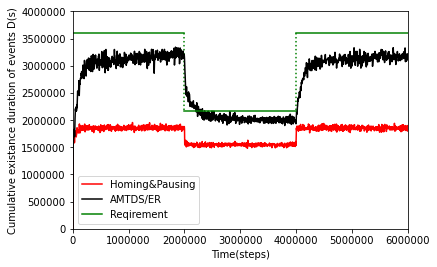
\includegraphics[width=0.9\hsize]{figures/ds_graph_3600_ave_ER_Office_600&1000.png}
    \caption{$D(s)$の時間推移(実験3)}
    \label{fig:ds_ER_ChangeRequirement}
    \hfill
    \centering
    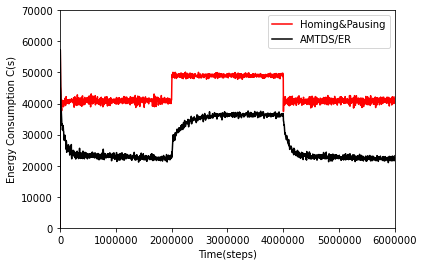
\includegraphics[width=0.9\hsize]{figures/cs_graph_3600_ave_ER_Office_600&1000.png}
    \caption{$C(s)$の時間推移(実験3)}
    \label{fig:cs_ER_ChangeRequirement}
  \end{figure}

  \begin{figure}
    \centering
    \begin{minipage}{0.85\columnwidth}
      \centering
      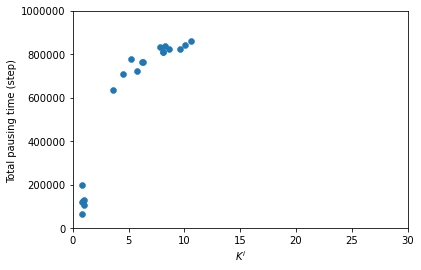
\includegraphics[width=0.8\hsize]{figures/CorrectionScatter_ChangeRequirement_2m.png}
      \caption{エージェントごとの$K^i$と待機時間の関係(実験3:2,000,000)}
      \label{fig:cscatter_ChangeRequirement_2m}
    \end{minipage}
    \vskip\baselineskip
    \begin{minipage}{0.85\columnwidth}
      \centering
      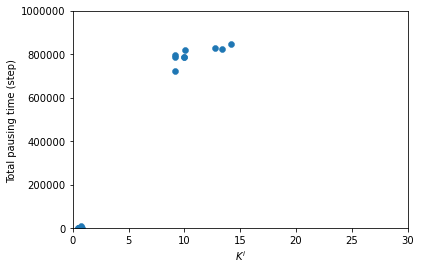
\includegraphics[width=0.8\hsize]{figures/CorrectionScatter_ChangeRequirement_4m.png}
      \caption{エージェントごとの$K^i$と待機時間の関係(実験3:4,000,000)}
      \label{fig:cscatter_ChangeRequirement_4m}
    \end{minipage}
    \vskip\baselineskip
    \begin{minipage}{0.85\columnwidth}
      \centering
      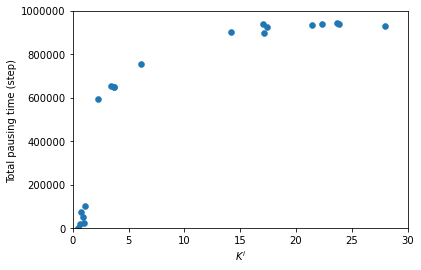
\includegraphics[width=0.8\hsize]{figures/CorrectionScatter_ChangeRequirement_6m.png}
      \caption{エージェントごとの$K^i$と待機時間の関係(実験3:6,000,000)}
      \label{fig:cscatter_ChangeRequirement_6m}
    \end{minipage}
  \end{figure}

  \begin{figure}
    \centering
    \begin{minipage}{0.85\columnwidth}
      \centering
      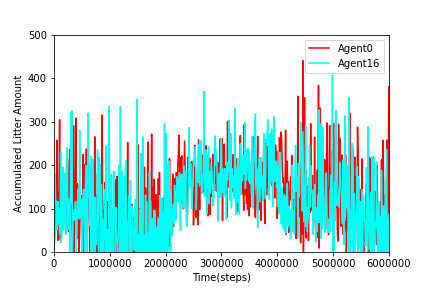
\includegraphics[width=0.75\hsize]{figures/al_graph_ER_ChangeRequirement_dual.png}
      \caption{エージェントのイベント処理数の時間推移(全期間ともグループ変更)}
      \label{fig:al_ChangeRequirement_dual}
    \end{minipage}
    \vskip\baselineskip
    \begin{minipage}{0.85\columnwidth}
      \centering
      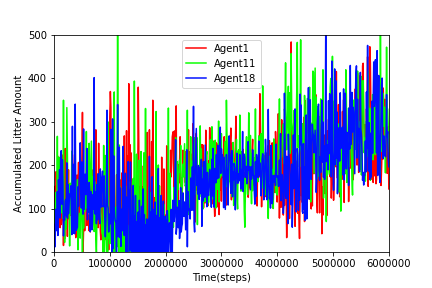
\includegraphics[width=0.75\hsize]{figures/al_graph_ER_ChangeRequirement_first.png}
      \caption{エージェントのイベント処理数の時間推移(P1$\sim$P2でグループ変更)}
      \label{fig:al_ChangeRequirement_first}
    \end{minipage}
    \vskip\baselineskip
    \begin{minipage}{0.85\columnwidth}
      \centering
      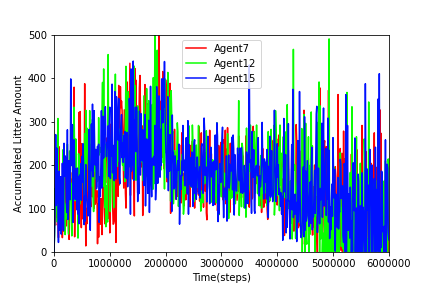
\includegraphics[width=0.75\hsize]{figures/al_graph_ER_ChangeRequirement_second.png}
      \caption{エージェントのイベント処理数の時間推移(P2$\sim$P3でグループ変更)}
      \label{fig:al_ChangeRequirement_second}
    \end{minipage}
  \end{figure}

  
  \subsubsection{実験3: $\Dreq$の変化による性能の変化}\label{ex:ER3}
  この項では,要求値$\Dreq$が途中で変化した際に,提案手法は対応できるのかを検証する.
  図\ref{fig:ds_ER_ChangeRequirement},\ref{fig:cs_ER_ChangeRequirement}は環境2で実験を行い,
  それぞれ3,600ステップごとの$D(s)$と$C(s)$の時間推移を示したものである.
  ここで,$0 \sim 2,000,000$ステップの期間をP1,$4,000,000 \sim 6,000,000$ステップの期間をP2,
  $4,000,000 \sim 6,000,000$ステップの期間をP3として,
  $\Dreq$はP1とP3では1,000であり,P2では600と設定している.
  つまり,エージェントはP1とP3では$D(s) \leq 3,600,000 (= 3600\Dreq)$を保ち,
  P2では$D(s) \leq 2,160,000 (= 3600\Dreq)$を保つことが要求条件であることに注意されたい.
  図\ref{fig:ds_ER_ChangeRequirement}より,提案手法であるAMTDS/ERは,
  途中で品質要求が変化してもしっかり対応できていることがわかる.
  従来手法であるAMTDS/ESCも$\Dreq$が変化した際に$D(s)$を変化させているが,
  その変化量は$\Dreq$の変化量と比べると小さい.
  このことから,エネルギー節約行動を調整する学習パラメータ$K^i$の導入により,
  品質要求の変化にも対応できたといえる.
  \par

  次に,$\Dreq$が変化したときの各エージェントの学習パラメータ$K^i$と,
  {\em Pausing}による待機時間の関係をまとめた散布図が図\ref{fig:cscatter_ChangeRequirement_2m}
  $\sim$\ref{fig:cscatter_ChangeRequirement_6m}である.
  なお,それぞれは2,000,000ステップ,4,000,000ステップ,6,000,000ステップ時点での$K^i$と,
  直前1,000,000ステップにおける待機時間の総和をプロットしてある.
  これらの図より,品質要求によってプロットの散らばりぐらいが異なることが分かる.
  $\Dreq$が小さくなると厳しくなった品質要求を満たすために,$K^i$が小さくなり,
  待機時間が短くなって巡回を多く行うようになったエージェントが存在し,
  $\Dreq$が大きくなると品質要求に対して巡回が過剰であるため,$K^i$が大きくなり,
  待機時間が長くなったエージェントが存在することが分かる.
  また,それぞれの図でのB-goupとES-groupのエージェント数は,
  図\ref{fig:cscatter_ChangeRequirement_2m}では6体と14体,
  図\ref{fig:cscatter_ChangeRequirement_4m}では11体と9体,
  図\ref{fig:cscatter_ChangeRequirement_6m}では6体と14体であった.
  \par

  さらに,図\ref{fig:al_ChangeRequirement_dual}$\sim$\ref{fig:al_ChangeRequirement_second}に,
  P1$\sim$P3の期間でB-groupとES-groupのうち,属するグループを変更したエージェントのイベント処理数の時間推移を示す.
  なお,図\ref{fig:al_ChangeRequirement_dual}はP1$\sim$P2とP2$\sim$P3のどちらでも属するグループを変更したエージェントであり,
  図\ref{fig:al_ChangeRequirement_first}はP1$\sim$P2で,
  図\ref{fig:al_ChangeRequirement_second}はP1$\sim$P2で属するグループを変更したエージェントを示している.
  まず,図\ref{fig:al_ChangeRequirement_dual}にプロットしたエージェントは,P1$\sim$P2ではES-groupからB-groupに,
  P2$\sim$P3ではB-groupからES-groupに変更した.
  これは,イベント処理数の時間推移からも確認することができる.
  P1とP3ではES-groupに属しているため,図\ref{fig:al_ER_Office_top}のように,時間とともに待機時間が増え,イベント処理数が減少しているが,
  P2ではB-groupに属しているため,図\ref{fig:al_ER_Office_least}のように,ES-groupの分もイベント処理している.
  次に,図\ref{fig:al_ChangeRequirement_first}にプロットしたエージェントは,P1$\sim$P2でES-groupからB-groupに変更した.
  実際に,図\ref{fig:fig:al_ChangeRequirement_first}では,P1はイベント処理数が減少しているが,
  P2とP3ではES-groupの分もイベントを処理するようになり,イベント処理数を増加させている.
  さらに,図\ref{fig:al_ChangeRequirement_second}にプロットしたエージェントは,P2$\sim$P3でB-groupからES-groupひ変更した.
  これまでと同様に,図\ref{fig:al_ChangeRequirement_second}より,P1ではイベント処理数を増加させ,
  P2では品質要求が厳しくなったことによって,B-groupに属するエージェントが増えたため,
  イベント処理数はP1よりは少ないが,一定量を維持し,
  P3ではイベント処理数が減少していることを確認することができる.
  \par

  以上より,提案手法であるAMTDS/ERは,品質要求が世中で変化しても対応でき,
  それに応じて2つのグループの構成比を変化させることができる手法であるといえる.


  \begin{figure}
    \centering
    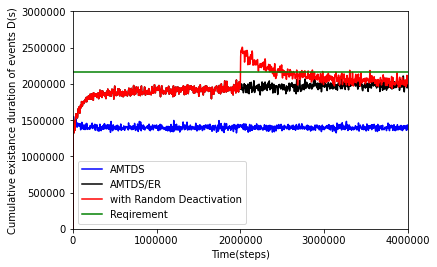
\includegraphics[width=0.9\hsize]{figures/ds_graph_3600_ave_ER_Office_randomStop.png}
    \caption{ランダム停止における$D(s)$の時間推移(実験4)}
    \label{fig:ds_RandomStop}
    \vspace{12pt}
    \centering
    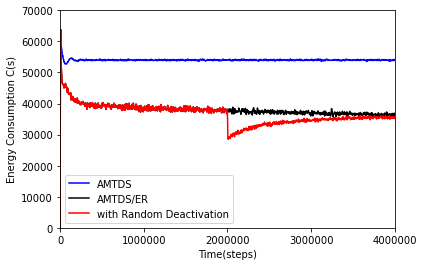
\includegraphics[width=0.9\hsize]{figures/cs_graph_3600_ave_ER_Office_randomStop.png}
    \caption{ランダム停止における$C(s)$の時間推移(実験4)}
    \label{fig:cs_RandomStop}
  \end{figure}

  \begin{figure}
    \begin{minipage}{0.48\hsize}
      \centering
      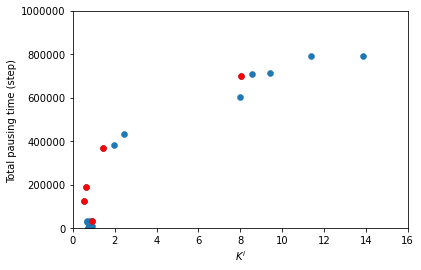
\includegraphics[width=0.99\hsize]{figures/CorrectionScatter_Office_RandomStop_before.png}
      \subcaption{停止時}
      \label{subfig:cscatter_RandomStop_before}  
    \end{minipage}
    \hfill
    \begin{minipage}{0.48\hsize}
      \centering
      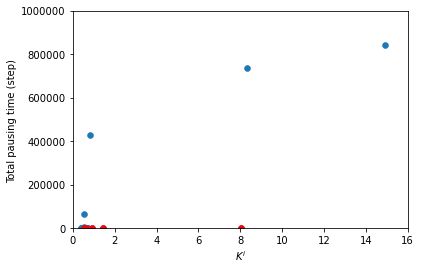
\includegraphics[width=0.99\hsize]{figures/CorrectionScatter_Office_RandomStop_after.png}
      \subcaption{停止後}
      \label{subfig:cscatter_RandomStop_after}  
    \end{minipage}
    \caption{エージェントごとの$K^i$と待機時間の関係(ランダム停止)}
    \label{fig:cscatter_RandomStop}
  \end{figure}

  \begin{figure}
    \begin{minipage}{0.48\hsize}
      \centering
      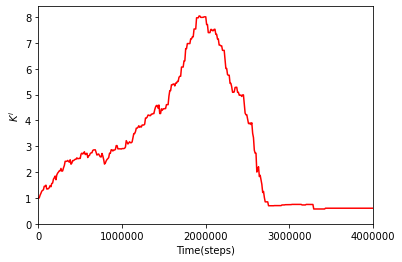
\includegraphics[width=0.99\hsize]{figures/CorrectionTransition_RandomStop_10.png}
      \subcaption{停止後にB-groupになったエージェント}
      \label{subfig:transition_random_10}
    \end{minipage}
    \hfill
    \begin{minipage}{0.48\hsize}
      \centering
      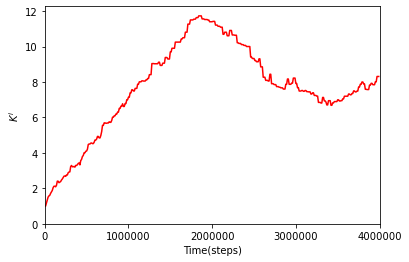
\includegraphics[width=0.99\hsize]{figures/CorrectionTransition_RandomStop_7.png}
      \subcaption{停止後もES-groupであったエージェント}
      \label{subfig:transition_random_7}
    \end{minipage}
    \caption{エージェントの$K^i$の時間推移(ランダム停止)}
    \label{fig:transition_randomStop}
  \end{figure}

  \begin{figure}
    \centering
    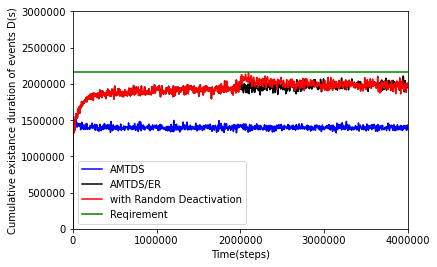
\includegraphics[width=0.9\hsize]{figures/ds_graph_3600_ave_ER_Office_descendingStop.png}
    \caption{降順停止における$D(s)$の時間推移(実験4)}
    \label{fig:ds_DescendingStop}
    \vspace{12pt}
    \centering
    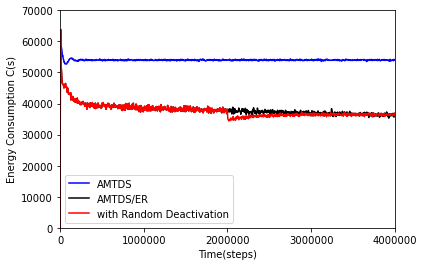
\includegraphics[width=0.9\hsize]{figures/cs_graph_3600_ave_ER_Office_descendingStop.png}
    \caption{降順停止における$C(s)$の時間推移(実験4)}
    \label{fig:cs_DescendingStop}
  \end{figure}

  \begin{figure}
    \begin{minipage}{0.48\hsize}
      \centering
      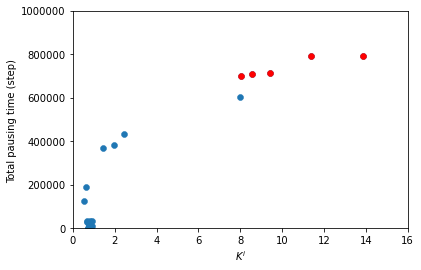
\includegraphics[width=0.99\hsize]{figures/CorrectionScatter_Office_DescendingStop_before.png}
      \subcaption{停止時}
      \label{subfig:cscatter_DescendingStop_before}  
    \end{minipage}
    \hfill
    \begin{minipage}{0.48\hsize}
      \centering
      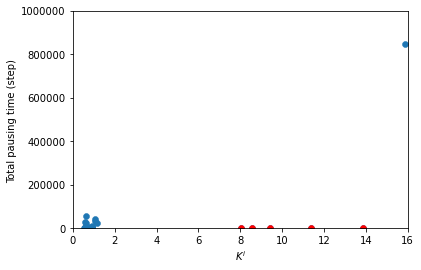
\includegraphics[width=0.99\hsize]{figures/CorrectionScatter_Office_DescendingStop_after.png}
      \subcaption{停止後}
      \label{subfig:cscatter_DescendingStop_after}  
    \end{minipage}
    \caption{エージェントごとの$K^i$と待機時間の関係(降順停止)}
    \label{fig:cscatter_DescendingStop}
  \end{figure}

  \begin{figure}
    \begin{minipage}{0.48\hsize}
      \centering
      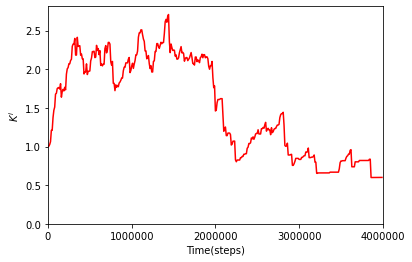
\includegraphics[width=0.99\hsize]{figures/CorrectionTransition_DescendingStop_2.png}
      \subcaption{停止後もB-groupであったエージェント}
      \label{subfig:transition_descending_2}
    \end{minipage}
    \hfill
    \begin{minipage}{0.48\hsize}
      \centering
      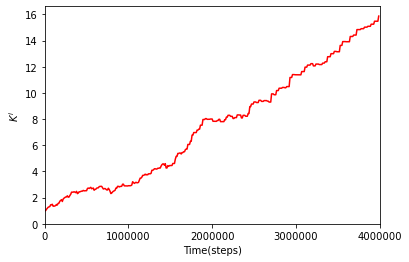
\includegraphics[width=0.99\hsize]{figures/CorrectionTransition_DescendingStop_10.png}
      \subcaption{停止後もES-groupであったエージェント}
      \label{subfig:transition_descending_10}
    \end{minipage}
    \caption{エージェントの$K^i$の時間推移(降順停止)}
    \label{fig:transition_descendingStop}
  \end{figure}
  

  \subsubsection{実験4: エージェント数減少による性能の変化}\label{ex:ER4}
  この節では,途中でエージェントが複数体停止したとき,提案手法のAMTDS/ERが品質要求を満たさせるかを検証する.
  ここでは,2,000,000ステップで5体停止させ,ランダムに5体停止と$K^i$の降順に5体停止の2つの停止手法を比較する.
  前者は巡回中のエージェントの故障を想定し,
  後者はエージェント数を減らしたいときに{\em Pausing}による待機を多めにしているエージェントから停止する状況を想定している.
  \par

  図\ref{fig:ds_RandomStop},\ref{fig:cs_RandomStop}は,環境1でランダムに5体停止を行い,
  それぞれ3,600ステップごとの$D(s)$と$C(s)$を示したものである.
  図\ref{fig:ds_RandomStop}より,2,000,000ステップでランダムに5体停止したため,
  $D(s)$の一時的な悪化が生じてしまい,品質要求を満たすことができなくなってしまっている.
  しかし,その後徐々に品質要求を満たせるようになった.
  \par

  図\ref{subfig:cscatter_RandomStop_before}は2,000,000ステップ時点での$K^i$と,
  1,000,000$\sim$2,000,000ステップでの総待機時間をプロットしたものであり,
  この時に停止するエージェントを赤でプロットしている.
  この図より,停止するエージェントは,待機時間が少ないものもあれば,多いものもあることが分かる.
  つまり,停止エージェントはB-groupやES-groupに偏らずに選択された.
  次に,図\ref{subfig:cscatter_RandomStop_after}は4,000,000ステップ時点での$K^i$と,
  3,000,000$\sim$4,000,000ステップでの総待機時間をプロットしたものである.
  図\ref{subfig:cscatter_RandomStop_before},\ref{subfig:cscatter_RandomStop_after}より,
  品質要求を満たすために待機時間が短く,巡回中心であったエージェントが停止し,
  このままでは品質要求をみたせないため,その時は待機時間が長かったエージェントも$K^i$が小さくなり,
  待機時間も短くなったことが分かる.
  \par

  また,図\ref{fig:transition_randomStop}はエージェントの$K^i$の時間推移を示したものである.
  図\ref{subfig:transition_random_10}はランダム停止後に,品質要求を満すためにES-groupからB-goupになったエージェントであり,
  図\ref{subfig:transition_random_7}はランダム停止後もES-groupのままであったエージェントである.
  図\ref{subfig:transition_random_10}より,このエージェントは停止後に品質要求が満たさなくなったと判断し,
  元々は$K^i$が大きかったのに,停止後に急激に減少し,B-goupになり,巡回中心になったことが分かる.
  一方,図\ref{subfig:transition_random_7}より,このエージェントも停止後は品質要求が満たさなくなったと判断し,
  $K^i$を減少させたが,他のエージェントも巡回を多くしたため品質要求が満たさせるようになり,
  エネルギー消費抑制の観点から,ES-groupのままであったということが分かる.
  \par

  以上より,ランダムにエージェントを停止した際,$D(s)$の一時的な悪化は起きてしまうものの,
  その後にエージェントが品質要求を満たさせていないと判断し,$K^i$を変化させ,
  B-groupとES-groupの比率を変化させることにより,品質要求を満たせるようになった.
  つまり,提案手法のAMTDS/ERは,巡回中にエージェントが故障し停止してしまっても,
  学習パラメータ$K^i$を変化させることにより,対応できるということが分かった.
  \par
  
  図\ref{fig:ds_DescendingStop},\ref{fig:cs_DescendingStop}は,環境1で$K^i$の降順に5体停止を行い,
  それぞれ3,600ステップごとの$D(s)$と$C(s)$を示したものである.
  図\ref{fig:ds_RandomStop}と図\ref{fig:ds_DescendingStop}を比較すると,前述したランダム停止と比べて,
  停止時の$D(s)$の一時的な悪化がかなり緩和されていることが分かる.
  具体的には,ランダム停止時のピークから降順停止のピークは,約13.9\%削減することができた.
  ランダム停止では品質要求を大幅に超えてしまっていたが,降順停止では停止による悪化をかなり抑え,
  品質要求も満たせたままでいることができた.
  \par
  
  次に,図\ref{subfig:cscatter_DescendingStop_before}は2,000,000ステップ時点での$K^i$と,
  1,000,000$\sim$2,000,000ステップでの総待機時間をプロットしたものであり,
  この時に停止するエージェントは赤でプロットしている.
  この図より,停止するエージェントは,$K^i$が大きいものから5体選べていることが分かる.
  また,図\ref{subfig:cscatter_DescendingStop_after}は4,000,000ステップ時点での$K^i$と,
  3,000,000$\sim$4,000,000ステップでの総待機時間をプロットしたものである.
  図\ref{subfig:cscatter_DescendingStop_before},\ref{subfig:cscatter_DescendingStop_after}より,
  $K^i$の大きなエージェントが停止したため,停止後にES-groupからB-groupに変更したエージェントは少なかった.
  これは,元々待機時間が多くイベント処理をあまり行っていなかったエージェントが停止したため,
  それをカバーするのは容易であり,ランダム停止に比べて,
  待機時間を減らして巡回を多くやる必要があまりなかったからだと考えられる.
  \par

  また,図\ref{fig:transition_descendingStop}はエージェントの$K^i$の時間推移を示したものである.
  降順停止では,前述したランダム停止と比べて,停止後に大きな役割の変更はなかった.
  しかし,同じ役割でも$K^i$の変化から,行動の変化を読み取ることができる.
  図\ref{subfig:transition_descending_2}は,停止前後でもB-groupであったエージェントであり,
  図\ref{subfig:transition_descending_10}は,停止前後でもES-groupであったエージェントである.
  図\ref{subfig:transition_descending_2}より,このエージェントは停止前も$K^i$が小さく,
  B-groupであったが,2,000,000ステップで降順停止後はさらに$K^i$を小さくしている.
  これにより,停止前は待機時間をある程度とっていたが,停止後はほとんど待機せずに巡回するようになった.
  一方,図\ref{subfig:transition_descending_10}より,このエージェントは停止前から$K^i$が大きく,
  停止後も$K^i$が増加している.
  しかし,2,000,000ステップでの停止直後はほとんど増加していない.
  つまり,この期間では品質要求を満たすために,
  停止していないエージェント達は図\ref{subfig:transition_descending_2}のように$K^i$を減少させ,
  停止したエージェントの分も巡回を行おうとする.
  それにより品質要求は十分に満たされ,これ以上待機時間を減らして巡回しなくても良くなり,
  エネルギー抑制の観点から,$K^i$を減らさずに増加を続け,待機時間を多くするということを判断していると考えられる.
  \par

  以上より,エージェント数を減らしたいときには,提案手法で導入した学習パラメータ$K^i$の降順に停止することにより,
  $D(s)$の一時的な悪化を最小限に留めることができるということが分かった.


  \begin{figure}
    \centering
    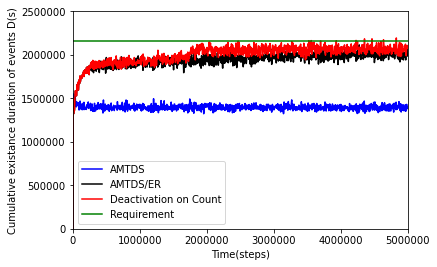
\includegraphics[width=0.9\hsize]{figures/ds_graph_3600_ave_CountStop_Office_600.png}
    \caption{$D(s)$の時間推移(実験5)}
    \label{fig:ds_CountStop}
    \vspace{12pt}
    \centering
    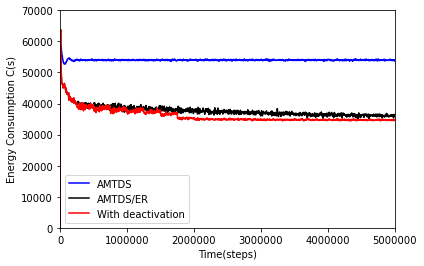
\includegraphics[width=0.9\hsize]{figures/cs_graph_3600_ave_CountStop_Office_600.png}
    \caption{$C(s)$の時間推移(実験5)}
    \label{fig:cs_CountStop}
  \end{figure}


  \subsection{不要なエージェントの停止}\label{ex:deactivation}
  この節では,\ref{sec:deactivation}節で述べたDeactivation on CountとDeactivation on Timeそれぞれの手法による,
  品質要求を満たす上で不要なエージェントを停止する実験を停止なしのAMTDS/ERと比較する.

  \subsubsection{実験5: Deactivation on Countによる不要なエージェントの停止}\label{ex:ER5}
  この項では,\ref{sec:expAnalsis}項での分析に基づき,
  \ref{sec:CountStop}項で述べたDeactivation on Countによる不要なエージェントの停止手法を評価するために,
  実験1と同じ設定で実験を行った.
  すなわち,品質要求を満たしながら,巡回エージェントの数を減らし,エネルギー消費を抑えられるかを検証する.
  表\ref{tb:4}に示すように,$\DeactCheckInterval=250,000$ごとにエージェントを停止できるかを確認した.
  \par

  図\ref{fig:ds_CountStop},\ref{fig:cs_CountStop}はそれぞれ$D(s)$と$C(s)$の
  5,000,000ステップまでの時間推移を示しており,
  図内のDeactivation on CountというラベルがDeactivation on Countによる停止手法を用いたAMTDS/ERを示している.
  この実験では,停止したエージェントの数は6から8の間であり,ほとんどが7であった.
  ここで,$D(s)$と$C(s)$の値は小さい方が良いことに再度注意されたい.
  \par

  図\ref{fig:ds_CountStop}より,Deactivation on Countを用いたAMTDS/ERは,
  停止手法を用いないAMTDS/ERと比較して,差は小さいが,
  品質要求を満たしつつ$D(s)$をより大きいことが分かる.
  これは,AMTDS/ERが既に$D(s)$の値を要求品質付近に維持できるためである.
  また,それにより図\ref{fig:cs_CountStop}より,エネルギー消費が若干減少した.
  しかし,停止手法ありと停止手法なしとの大きな違いは,停止したエージェントが巡回のタスクを
  他のエージェントに完全に移譲できている点である.
  さらに,$D(s)$と$C(s)$の性能差が大きくないにもかかわらず,
  以下のようなメリットがあることを強調したい.
  %
  \begin{enumerate}
    \item[(1)] 停止したエージェントを他の環境で利用できる
    \item[(2)] それらのエージェントを待機させ,巡回エージェントが故障時に利用できる
    \item[(3)] 定期点検や交代運用を行ってシステムを延命できる
  \end{enumerate}
  %


  \begin{figure}
    \centering
    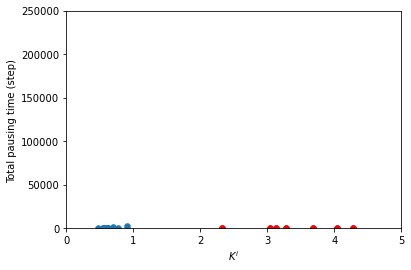
\includegraphics[width=0.8\hsize]{figures/CorrectionScatter_Office_CountStop.png}
    \caption{エージェントごとの$K^i$と待機時間の関係(実験5)}
    \label{fig:cscatter_CountStop_Office}
  \end{figure}

  \begin{figure}
    \begin{minipage}{0.48\hsize}
      \centering
      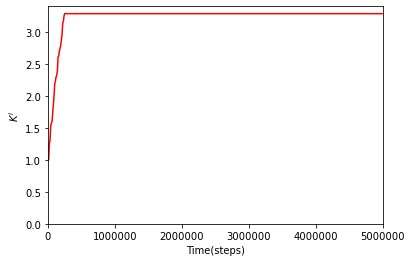
\includegraphics[width=0.99\hsize]{figures/CorrectionTransition_CountStop_18.png}
      \subcaption{$D= 250,000$ステップ}
      \label{subfig:transition_count_18}
    \end{minipage}
    \hfill
    \begin{minipage}{0.48\hsize}
      \centering
      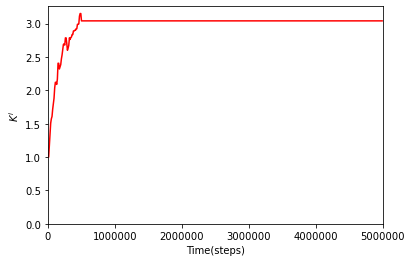
\includegraphics[width=0.99\hsize]{figures/CorrectionTransition_CountStop_7.png}
      \subcaption{$D=500,000$ステップ}
      \label{subfig:transition_count_7}
    \end{minipage}
    \caption{$D$ステップで停止したエージェントの$K^i$の時間推移(実験5)}
    \label{fig:transition_early_count}
  \vspace{12pt}
    \begin{minipage}{0.48\hsize}
      \centering
      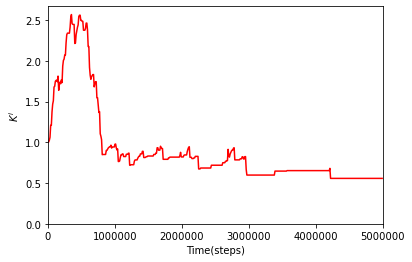
\includegraphics[width=0.99\hsize]{figures/CorrectionTransition_CountStop_2.png}
      \subcaption{例1}
      \label{subfig:transition_count_2}
    \end{minipage}
    \hfill
    \begin{minipage}{0.48\hsize}
      \centering
      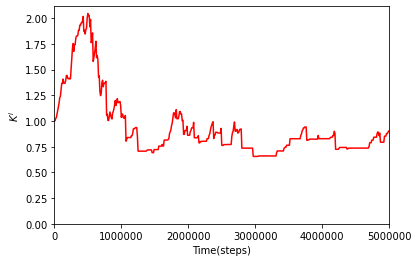
\includegraphics[width=0.99\hsize]{figures/CorrectionTransition_CountStop_9.png}
      \subcaption{例2}
      \label{subfig:transition_count_9}
    \end{minipage}
    \caption{非停止エージェントの$K^i$の時間推移(実験5)}
    \label{fig:transition_notSuspend_count}
  \end{figure}

  \subsubsection{実験5における停止エージェントと非停止エージェントの行動の解析}\label{sec:ex5Analsis}
  この項では,実験5における$K^i$の推移を調べることで,Deactivation on Countによる
  停止エージェントと非停止エージェントの行動を解析する.
  図\ref{fig:cscatter_CountStop_Office}に,実験5からランダムに選んだ,独立した1つの実験における
  $K^i$と$i$の{\em Pausing}による待機時間の関係をプロットする.
  ここで,$K^i$は5,000,000ステップでの値であり,待機時間は実験の最後の1,000,000ステップでの待機時間の総和である.
  したがって,停止したエージェント$i$の$K^i$は停止したときの値であり,
  待機時間は0である.
  図\ref{fig:cscatter_CountStop_Office}での7つの赤いプロットが停止エージェントに対応する.
  この図より,停止エージェントは$K^i$が比較的大きく,
  非停止エージェントは非常に短い待機時間で巡回を続けていることが分かる.
  このことから,この環境では13体のエージェントで要求品質を満たすことができたと考えられる.
  \par

  図\ref{fig:transition_early_count}と図\ref{fig:transition_notSuspend_count}は,
  250,000ステップと500,000ステップで停止したエージェント(図\ref{fig:transition_early_count})と,
  非停止エージェント(図\ref{fig:transition_notSuspend_count})の$K^i$の時間推移をプロットしたものである.
  図\ref{fig:transition_early_count}より,これらのエージェントの$K^i$は急激に増加し,
  待機時間がその時点で最大であったため,停止の対象に選ばれたことが分かる.
  停止後は$K^i$は変化しない.
  一方,非停止エージェントは一時的に$K^i$を増加させたが,
  その後,一部のエージェントが停止したため,$K^i$が減少し,
  比較的小さい値を維持した.
  つまり,非停止エージェントは品質要求を満たすために,
  停止エージェントの分も巡回しなければならなくなった.
  \par

  実験の結果,AMTDS/ERで導入した学習パラメータ$K^i$により,この値に基づき,
  さらに,関数\textsf{PLength}が呼び出された回数を比較してすることによって,
  巡回エージェントの数を削減することができた.

  
  \begin{figure}
    \centering
    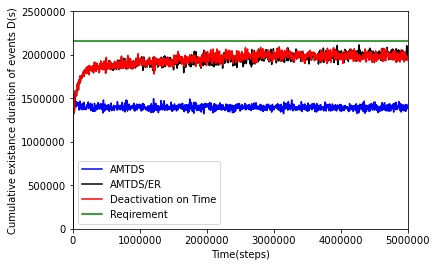
\includegraphics[width=0.9\hsize]{figures/ds_graph_3600_ave_TimeStop_Office_600.png}
    \caption{$D(s)$の時間推移(実験6)}
    \label{fig:ds_TimeStop}
    \vspace{12pt}
    \centering
    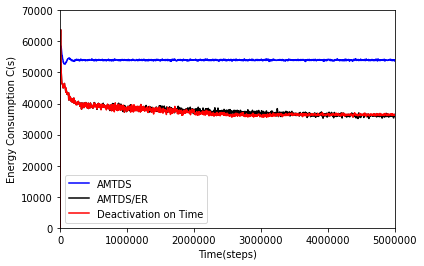
\includegraphics[width=0.9\hsize]{figures/cs_graph_3600_ave_TimeStop_Office_600.png}
    \caption{$C(s)$の時間推移(実験6)}
    \label{fig:cs_TimeStop}
  \end{figure}


  \subsubsection{実験6: Deactivation on Timeによる不要なエージェントの停止}\label{ex:ER6}
  この項では,\ref{sec:expAnalsis}項での分析に基づき,
  \ref{sec:TimeStop}で述べたDeactivation on Timeによる不要なエージェントの停止手法を評価するために,
  実験1と同じ設定で実験を行った.
  すなわち,品質要求を満たしながら,巡回エージェントの数を減らし,エネルギー消費を抑えられるかを検証する.
  表\ref{tb:4}に示すように,$\DeactCheckInterval = 250,000$ごとにエージェントを停止できるかを確認した.
  \par

  図\ref{fig:ds_TimeStop},\ref{fig:cs_TimeStop}はそれぞれ$D(s)$と$C(s)$の5,000,000ステップまでの時間推移を示しており,
  図内のDeactivation on TimeというラベルがDeactivation on Time による停止手法を用いたAMTDS/ERを示している.
  この実験では,停止したエージェントの数は5から7の間であり,ほとんどが6であった.
  ここで,$D(s)$と$C(s)$の値は小さい方がよいことに再度注意されたい.
  \par

  図\ref{fig:ds_TimeStop}より,Deactivation on Timeを用いたAMTDS/ERは,停止手法を用いないAMTDS/ERとほとんど差がなかった.
  それに伴い,図\ref{fig:cs_TimeStop}でも差が小さいのが分かる.
  つまり,システム全体の巡回性能をほとんど変化させることなく,エージェントの数を減らすことができた.
  ここでも,\ref{ex:ER5}項で述べた,停止手法によるメリットを再度強調したい.


  \begin{figure}
    \centering
    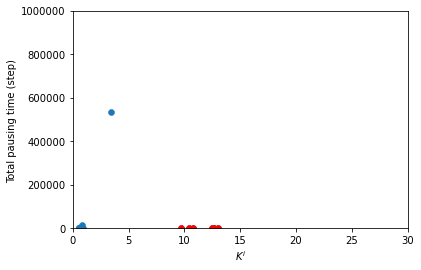
\includegraphics[width=0.8\hsize]{figures/CorrectionScatter_Office_TimeStop.png}
    \caption{エージェントごとの$K^i$と待機時間の関係(実験6)}
    \label{fig:cscatter_TimeStop_Office}
  \end{figure}

  \begin{figure}
    \begin{minipage}{0.48\hsize}
      \centering
      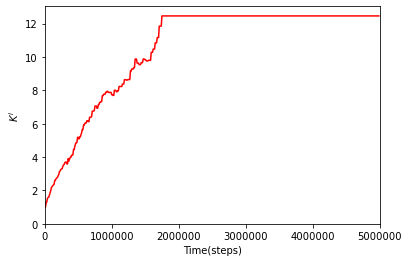
\includegraphics[width=0.99\hsize]{figures/CorrectionTransition_TimeStop_18.png}
      \subcaption{$D= 1,750,000$ステップ}
      \label{subfig:transition_time_18}
    \end{minipage}
    \hfill
    \begin{minipage}{0.48\hsize}
      \centering
      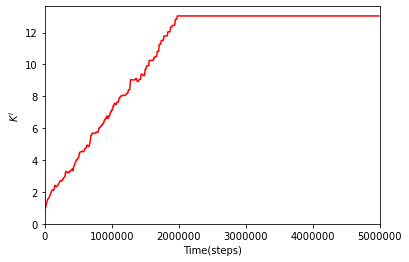
\includegraphics[width=0.99\hsize]{figures/CorrectionTransition_TimeStop_7.png}
      \subcaption{$D=2,000,000$ステップ}
      \label{subfig:transition_time_7}
    \end{minipage}
    \caption{$D$ステップで停止したエージェントの$K^i$の時間推移(実験6)}
    \label{fig:transition_early_time}
  \vspace{12pt}
    \begin{minipage}{0.48\hsize}
      \centering
      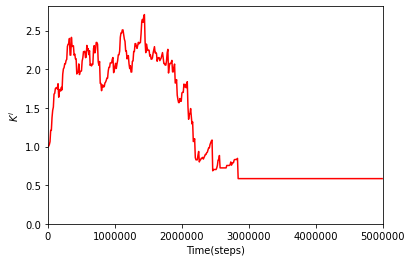
\includegraphics[width=0.99\hsize]{figures/CorrectionTransition_TimeStop_2.png}
      \subcaption{例1}
      \label{subfig:transition_time_2}
    \end{minipage}
    \hfill
    \begin{minipage}{0.48\hsize}
      \centering
      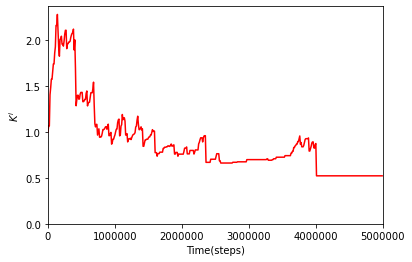
\includegraphics[width=0.99\hsize]{figures/CorrectionTransition_TimeStop_16.png}
      \subcaption{例2}
      \label{subfig:transition_time_16}
    \end{minipage}
    \caption{非停止エージェントの$K^i$の時間推移(実験6)}
    \label{fig:transition_notSuspend_time}
  \end{figure}

  \begin{figure}
    \centering
    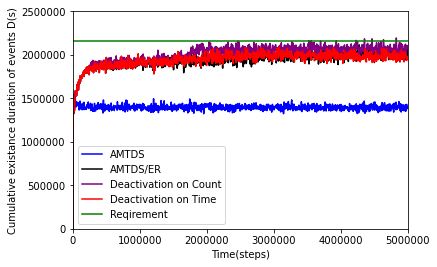
\includegraphics[width=0.9\hsize]{figures/ds_graph_3600_ave_CountTime_Office_600.png}
    \caption{$D(s)$の時間推移(Deactivation on CountとDeactivation on Time)}
    \label{fig:ds_CountTime}
    \vspace{12pt}
    \centering
    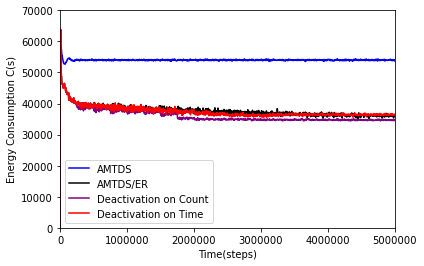
\includegraphics[width=0.9\hsize]{figures/cs_graph_3600_ave_CountTime_Office_600.png}
    \caption{$C(s)$の時間推移(Deactivation on CountとDeactivation on Time)}
    \label{fig:cs_CountTime}
  \end{figure}

  \begin{figure}
    \centering
    \includegraphics[width=0.9\hsize]{figures/ds_graph_3600_ave_TimeStop30_Office_600.png}
    \caption{$D(s)$の時間推移(30体)}
    \label{fig:ds_TimeStop30}
    \vspace{40pt}
    \centering
    \includegraphics[width=0.9\hsize]{figures/cs_graph_3600_ave_TimeStop30_Office_600.png}
    \caption{$C(s)$の時間推移(30体)}
    \label{fig:cs_TimeStop30}
  \end{figure}

  \begin{figure}
    \centering
    \includegraphics[width=0.8\hsize]{figures/CorrectionScatter_Office_TimeStop30.png}
    \caption{エージェントごとの$K^i$と待機時間の関係(30体)}
    \label{fig:cscatter_TimeStop30_Office}
  \end{figure}


  \subsubsection{実験6における停止エージェントと非停止エージェントの行動の解析}\label{sec:ex6Analsis}
  この項では,Deactivation on Timeによる停止エージェントと非停止エージェントの行動を解析し,
  実験5のDeactivation on Countと比較する.
  図\ref{fig:cscatter_TimeStop_Office}に,実験6からランダムに選んだ,
  独立した1つの実験における$K^i$と$i$の{\em Pausing}による待機時間の関係をプロットする.
  ここで,$K^i$は5,000,000ステップでの値であり,
  待機時間は実験の最後の1,000,000ステップでの待機時間の総和である.
  したがって,停止したエージェント$i$の$K^i$は停止したときの値であり,
  待機時間は0である.
  図\ref{fig:cscatter_TimeStop_Office}での6つの赤いプロットが停止エージェントに対応する.
  この図でも,停止エージェントは$K^i$が大きく,非停止エージェントは非常に短い待機時間で巡回を続けていることが分かる.
  また,待機時間が500,000以上であるが停止していないエージェントが1体確認することができる.
  これは,実験5では停止していたエージェントである.
  他の独立した実験でも,実験設定は同じであるが,停止したエージェント数はDeactivation on Countの方がDeactivation on Time以上であり,
  独立した50試行の平均では,1.1体多かった.
  つまり,Deactivation on Countでは,図\ref{fig:cscatter_CountStop_Office}のように,
  非停止エージェントの待機時間は0に近かったが,Deactivation on Timeでは,
  比較的待機時間が大きいエージェントが1体残ったという結果になった.
  しかし,停止手法の優劣を決める際に,停止したエージェント数が多いという点が必ずしも優先されるべきではない.
  実験5と実験6では,停止したエージェントが巡回を再開することはないため,
  停止をしすぎて品質要求を満たせないということはあってはならない.
  このような条件の際に,Deactivation on Timeでは\ref{sec:TimeStop}項で述べたように,
  しっかり役割分担が行われてから停止を始めるようにしており,エージェントを停止しても,
  そのエージェントの分の巡回を残りのエージェントでカバーすることができることが保証されてから停止をするようになっている.
  しかし,Deactivation on Countでは,現在のエージェント数では要求品質を十分に満たせていることは確認できているが,
  エージェントの停止によって,どの程度の影響があるかは確認できずに停止している.
  つまり,Deactivation on Countの方では,エージェントを停止しすぎてしまう可能性もある.
  図\ref{fig:ds_CountTime},\ref{fig:cs_CountTime}に
  Deactivation on CountとDeactivation on Timeの$D(s)$と$C(s)$の時間推移をプロットした.
  これらの図から分かるように,両者の巡回効率やエネルギー消費量はほとんど差がないことを考慮すると,
  停止手法としてより望ましいのはDeactivation on Timeの方であると考えられる.
  \par

  次に,実験6における$K^i$の推移を調べた.
  図\ref{fig:transition_early_time}と図\ref{fig:transition_notSuspend_time}は,
  1,750,000ステップと2,000,000ステップで停止したエージェント(図\ref{fig:transition_early_time})と,
  非停止エージェント(図\ref{fig:transition_notSuspend_time})の$K^i$の時間推移をプロットしたものである.
  式(\ref{eq:sillet})での平均シルエット係数$S$と閾値$S_{deact}$の比較のため,停止し始めた時刻は実験5よりも遅いが,
  大まかな結果は\ref{sec:ex5Analsis}項と同様である.
  停止エージェントは$K^i$が急激に増加し停止の対象に選ばれた一方で,
  非停止エージェントは一時的に$K^i$を増加させたが,一部のエージェントが停止したため,$K^i$が減少した.
  \par

  さらに,Deactivation on Timeでエージェント数$|A|$を30にして実験を行った.
  \\\red{図はAMTDS/ER(30)を追加して変更}\\
  \red{20台のDeactivation on Timeも追加してもいいかも}\\
  図\ref{fig:ds_TimeStop30},\ref{fig:cs_TimeStop30}はそれぞれ$D(s)$と$C(s)$の8,000,000ステップまでの時間推移を示している.
  この実験では,停止したエージェント数は16から18の間であり,ほとんどが17であった.
  図\ref{fig:ds_TimeStop30}より,エージェント数を変化させても,品質要求を満たすことができていることが分かる.
  \par

  次に,図\ref{fig:cscatter_TimeStop30_Office}に$K^i$と$i$の{\em Pausing}による待機時間の関係をプロットする.
  ここで,$K^i$は8,000,000ステップでの値であり,待機時間は実験の最後の1,000,000ステップでの待機時間の総和である.
  この図での17つの赤いプロットが停止エージェントに対応する.
  この図より,図\ref{fig:cscatter_TimeStop_Office}と同様に,比較的待機時間が大きいエージェントが1体残ったという結果となった.
  また,この実験では$|A|$以外の実験設定は変更していないため,品質要求を満たした上で停止するエージェント数は,
  単純に10体増えると予想したが,独立した50試行ではほとんどが停止エージェント数の差が11体であり,
  平均は11.02体であった.
  しかし,図\ref{fig:ds_TimeStop30}や図\ref{fig:cscatter_TimeStop30_Office}でも分かるように,
  エージェントを停止しすぎたわけではなく,品質要求を満たせている.
  これは最初に巡回していたエージェント数が増えたことにより,$|A|=20$の時よりもエージェントの役割が細分化され,
  エージェントの学習も異なったためであると考えられる.
  以上より,Deactivation on Timeではエージェント数が異なっても,
  品質要求を満たしながら不要なエージェントを最大限停止することができた.

  
  \subsection{AMTDS/ERCについての実験結果}\label{result_ERC}
  提案手法であるAMTDS/ERCについての評価実験を,
  エネルギー節約行動を行わないAMTDS/EDCと比較しながら行った.
  この節では,複数の条件下での実験結果を,評価指標である$D(s)$や$C(s)$,
  さらには,必要に応じて他の指標とも比較していく.
  なお,先行研究では$p^i(v)$を学習しながらエネルギー消費を抑制する手法はないため,
  比較手法はAMTDS/EDCだけということに注意されたい.


  \begin{figure}
    \centering
    \includegraphics[width=0.9\hsize]{figures/ds_graph_3600_ave_ERC_Office_600.png}
    \caption{$D(s)$の時間推移(実験7)}
    \label{fig:ds_ERC_Office}
    \vspace{40pt}
    \centering
    \includegraphics[width=0.9\hsize]{figures/cs_graph_3600_ave_ERC_Office_600.png}
    \caption{$C(s)$の時間推移(実験7)}
    \label{fig:cs_ERC_Office}
  \end{figure}

  
  \subsubsection{実験7: 性能評価}\label{ex:ERC1}
  \red{後で図を変更する}\\
  図\ref{fig:ds_ERC_Office},\ref{fig:cs_ERC_Office}は,
  それぞれ3,600ステップごとの$D(s)$と$C(s)$の時間推移を示したものである.
  なお,図\ref{fig:ds_ERC_Office}では$\Dreq=1,000$なので,
  エージェントは$D(s) \leq 3,600,000 (=3,600\Dreq)$を保つことが要求条件になることに注意されたい.
  図\ref{fig:ds_ERC_Office}より,提案手法は品質要求を満たせていることが分かる.
  AMTDS/ERCはAMTDS/EDCに比べて$D(s)$は約\red{??.?}増加したが,
  図\ref{fig:cs_ERC_Office}より,エネルギー節約行動を行わないAMTDS/EDCよりもエネルギー消費量を削減することができ,
  具体的には約\red{??.?}削減することができた.
  

  \begin{figure}
    \centering
    \includegraphics[width=0.9\hsize]{figures/ds_graph_3600_ave_ERC_Complex_600.png}
    \caption{$D(s)$の時間推移(実験8)}
    \label{fig:ds_ERC_Complex}
    \vspace{40pt}
    \centering
    \includegraphics[width=0.9\hsize]{figures/cs_graph_3600_ave_ERC_Complex_600.png}
    \caption{$C(s)$の時間推移(実験8)}
    \label{fig:cs_ERC_Complex}
  \end{figure}
  
   
  \subsubsection{実験8: 異なる環境による性能評価}\label{ex:ERC2}
  \red{$\Dreq=600$にして実験をしてみる}\\
  \red{図変更}\\
  図\ref{fig:ds_ERC_Complex},\ref{fig:cs_ERC_Complex}は,環境2で実験を行い,
  それぞれ3,600ステップごとの$D(s)$と$C(s)$の時間推移を示している.
  これらの図より,品質要求を満たしながらAMTDS/EDCよりもエネルギー消費量を削減することができた.
  しかし,実験7のように最大限削減できたとは言えない.
  $D(s)$は品質要求よりもまだ余裕があるため,要求条件よりも過剰な巡回を行ってしまっていると言える.

  環境によってエネルギー削減を最大限に行えないという点は,今後の課題である.


  \begin{figure}
    \begin{minipage}{1.0\columnwidth}
      \centering
      \includegraphics[width=0.8\hsize]{figures/CorrectionScatter_Office_ERC.png}
      \caption{エージェントごとの$K^i$と待機時間の関係(実験7)}
      \label{fig:cscatter_ERC_Office}
    \end{minipage}
    \\[40pt]
    \begin{minipage}{1.0\columnwidth}
      \centering
      \includegraphics[width=0.8\hsize]{figures/CorrectionScatter_Complex_ERC.png}
      \caption{エージェントごとの$K^i$と待機時間の関係(実験8)}
      \label{fig:cscatter_ERC_Complex}
    \end{minipage}
  \end{figure}



  \subsubsection{AMTDS/ERCの行動の解析}\label{sec:expAnalsisERC}
  \red{図変更}\\
  この項では,実験7と実験8でのエージェントの行動を解析し,提案手法はであるAMTDS/ERCを定性的に評価する.



  \iffalse
  \begin{figure}
    \centering
    \includegraphics[width=0.9\hsize]{figures/ds_graph_3600_ave_ERC_Office_randomStop.png}
    \caption{ランダム停止における$D(s)$の時間推移(実験8)}
    \label{fig:ds_ERC_RandomStop}
    \vspace{40pt}
    \centering
    \includegraphics[width=0.9\hsize]{figures/cs_graph_3600_ave_ERC_Office_randomStop.png}
    \caption{ランダム停止における$C(s)$の時間推移(実験8)}
    \label{fig:cs_ERC_RandomStop}
  \end{figure}

  \begin{figure}
    \centering
    \includegraphics[width=0.9\hsize]{figures/ds_graph_3600_ave_ERC_Office_descendingStop.png}
    \caption{降順停止における$D(s)$の時間推移(実験8)}
    \label{fig:ds_ERC_DescendingStop}
    \vspace{40pt}
    \centering
    \includegraphics[width=0.9\hsize]{figures/cs_graph_3600_ave_ERC_Office_descendingStop.png}
    \caption{降順停止における$C(s)$の時間推移(実験8)}
    \label{fig:cs_ERC_DescendingStop}
  \end{figure}



  \subsubsection{実験9: エージェント数減少による性能の変化}\label{ex:ERC3}
  \red{randomだと悪化を元に戻せないor戻すのに時間がかかる}\\
  \red{descendingだと全然影響がない.}\\
  \red{それは、$K^i$が大きすぎて、randomだと対応できないが、descendingだとほとんど止まっている状態なので、影響なし}\\
  \red{これからの課題も書く}
  \fi

  \section{結論}

  \clearpage
  \bibliographystyle{junsrt}
  \bibliography{ref}

\end{document}